\chapter{Experiments design and results}
\label{chap:expe}
\textit{In this Chapter I expose all details about the evaluation process of \posl{}, i.e., all experiments I perform. For each benchmark, I explain used strategies in the evaluation process and the used environments were the runs were performed (\textit{Curiosiphi} server). %, and eventually \textit{Grid5000}). 
I describe all the experiments and I expose a complete analysis of the obtained result.}
\vfill
\minitoc
\newpage

In this chapter I illustrate and analyze the versatility of \posl{} studying different ways to solve constraint problems based on local search meta-heuristics. 
I have chosen the \sgp, the \nqp, the \carrp{} and the \grp{} as benchmarks since they are challenging yet differently structured problems. In this Chapter I present formally each benchmark, I explain the structure of \posl's solvers that I have generated for experiments and present a detailed analysis of obtained results.

The experiments\footnote{\posl{} source code is available on GitHub:\href{https://github.com/alejandro-reyesamaro/POSL}{https://github.com/alejandro-reyesamaro/POSL}} 
were performed on an Intel\R{} Xeon\TM{} E5-2680 v2, 10$\times$4 cores, 2.80GHz. This server is called \textit{Coriosiphi} and is located at \textit{Laboratoire d'Informatique de Nantes Atlantique}, at the University of Nantes. Showed results are the means of 30 runs for each setup, presented in columns labeled {\bf T}, corresponding to the run-time in seconds, and {\bf It.} corresponding to the number of iterations; and their respective standard deviations ({\bf T(sd)} and {\bf It.(sd)}). In some tables, the column labeled \textbf{\% success} indicates the percentage of solvers finding a solution before reaching a time--out (5 minutes).

\modified{The experiments in this Chapter are multi-walk runs}. Parallel experiments use 40 cores for all problem instances. It is important to point out that \posl{} is not designed to obtain the best results in terms of performance, but to give the possibility of rapidly prototyping and studying different cooperative or non cooperative search strategies.

\modified{All benchmarks were coded using the \posl{} low-level framework in C++.}

\modified{First results using \posl{} to solve} constraint problems were published in \cite{Reyes-amaro} were we used \posl{} to solve the \sgp{} and study some communication strategies. It was the first version of \posl{}, therefore it was able to solve only relatively easy instances. However, the efficacy of the communication was showed using this tool.

\modified{With the next and more optimized version of \posl{}, I decide to start to perform more detailed studies using the benchmark mentioned before and some others.}

\section{Solving the \sgp}
\label{sec:golfers}

In this section I present the performed study using \sgp{} (\SGP) as a benchmark. The \commstr{} analyzed in here consists in applying a mechanism of cost descending acceleration, exchanging the current configuration between two solvers with different characteristics. Final obtained results show that this \commstr{} works pretty well for this problem.

\subsection{Problem definition}

The \sgp{} (\SGP) consists in scheduling $g\times p$ golfers into $g$ groups of $p$ players every week for $w$ weeks, such that two players play in the same group at most once. An instance of this problem can be represented by the triple $g-p-w$. This problem, and other closely related problems, arise in many practical applications such as encoding, encryption, and covering problems~\cite{Lardeux2014}. Its structure is very attractive, because it is very similar to other problems, like \textit{Kirkman's Schoolgirl Problem} and the \textit{Steiner Triple System}. %, so efficient modules to solve a broad range of problems can be built.

The cost function for this benchmark was implemented making an efficient use of the stored information about the cost of the previews configuration. Using integers to work with bit-flags, a table to store the information about the partners of each player in each week can be filled in $O\left(p^2\cdot g \cdot w\right)$. So, if a configuration has $n = (p\cdot g \cdot w)$ elements, this table can be filled in $O\left(p\cdot n\right)$. This table is filled from scratch only one time in the search process (I explain in the next section why). Then, every cost of a new configuration, is calculated based on this information and the performed changes between the new configuration and the stored one. This relative cost is calculated in $O\left(c\cdot g\right)$, where $c$ is the number of performed changed in the new configuration with respect to the stored one.

\subsection{Experiment design and results}

Here, I present the \as{} designed for this problem as well as concrete \oms{} composing the different solvers I have tested:

\begin{enumerate}
	\item Generation abstract module $I$:
	\subitem $I_{BP}$: Returns a random configuration $s$, respecting the structure of the problem, {\it i.e.}, the configuration is a set of $w$ permutations of the vector $[1..n]$, where $n=g\times p$.
	\item Neighborhood abstract modules $V$:
	\subitem $V_{std}$: Given a configuration, returns the neighborhood $\mathcal{V}\left(s\right)$ swapping players among groups.
	\subitem $V_{BAS}$: Given a configuration, returns the neighborhood $\mathcal{V}\left(s\right)$ swapping the most culprit player with other players from the same week. It is based on the {\it Adaptive Search} algorithm.
	\subitem $V_{BP}(p)$: Given a configuration, returns the neighborhood $V\left(s\right)$ by swapping the culprit player chosen for all $p$ randomly selected weeks with other players in the same week
	\item Selection abstract modules $S$:
	\subitem $S_{first}$: Given a neighborhood, selects the first configuration $s' \in V\left(s\right)$ improving the current cost and returns it together with the current one, into a \textit{decision--pair}
	\subitem $S_{best}$: Given a neighborhood, selects the best configuration $s' \in V\left(s\right)$ improving the current cost and returns it together with the current one, into a \textit{decision--pair}
	\subitem $S_{rand}$: Given a neighborhood, selects randomly a configuration $s' \in V\left(s\right)$ and returns it together with the current one, into a \textit{decision--pair}.
	\item Acceptance abstract module $A$:
	\subitem $A_{AI}$: Given a decision--pair, returns the configuration marked as \textit{"found"}
\end{enumerate}

These concrete modules are very useful and can be reused to solve tournament-like problems like \textit{Sports Tournament Scheduling}, \textit{Kirkman's Schoolgirl} and the \textit{Steiner Triple System} problems.

In a first stage of the experiments I use the operator-based language provided by \posl{} to build and test many different non communicating strategies. The goal is to select the best concrete modules to run tests performing communication. A very first experiment was performed to select the best neighborhood function to solve the problem, comparing a basic solver using $V_{std}$; a new solver using $V_{BAS}$; and a combination of $V_{std}$ and $V_{BAS}$ by applying the operator $\circled{$\rho$}$, already introduced in the previous chapter. Algorithms~\ref{as:golfers10-10-3} and \ref{as:golfers_rho} present solvers for each case, respectively.

\begin{algorithm}[t]
\dontprintsemicolon
\SetNoline
\SetKwProg{myproc}{\tet{\bf abstract solver}}{\tet{\bf begin}}{\tet{\bf end}}
\myproc{as\_simple \tcp*{{\sc Itr} $\rightarrow$ number of iterations}
	\tet{\bf computation} : $I, V, S, A$\;}{
	\whileinline{$\left(\textbf{\Iter < } K_1\right)$}{%M_1^a \circled{$\rho$} M_1^b
		$I \poslop{\mapsto}$
		\whileinline{$\left(\textbf{\Iter \% } K_2\right)$}{$\left[V \poslop{\mapsto} S \poslop{\mapsto} A\right]$}
	}	
}
\tet{\bf solver} S\_std \tet{\bf implements} as\_simple\;
\algoindent \tet{\bf computation} : $I_{BP}, V_{std}, S_{best}, A_{AI}$ \;
\tet{\bf solver} S\_as \tet{\bf implements} as\_simple\;
\algoindent \tet{\bf computation} : $I_{BP}, V_{BAS}, S_{best}, A_{AI}$ \; 
%\tet{\bf connection}: $CM_{last}$\;
\caption{Simple solvers for \SGP}\label{as:golfers10-10-3}
\end{algorithm}

\begin{algorithm}[H]
\dontprintsemicolon
\SetNoline
\SetKwProg{myproc}{\tet{\bf abstract solver}}{\tet{\bf begin}}{\tet{\bf end}}
\myproc{as\_rho \tcp*{{\sc Itr} $\rightarrow$ number of iterations}
	\tet{\bf computation} : $I, V_1, V_2, S, A$\;}{
	\whileinline{$\left(\textbf{\Iter < } K_1\right)$}{%M_1^a \circled{$\rho$} M_1^b
		$I \poslop{\mapsto}$
		\whileinline{$\left(\textbf{\Iter \% } K_2\right)$}{$\left[\left[V_1 \poslop{\rho} V_2\right] \poslop{\mapsto} S \poslop{\mapsto} A\right]$}
	}	
}
\tet{\bf solver} S\_rho \tet{\bf implements} as\_rho\;
\algoindent \tet{\bf computation} : $I_{BP}, V_{std}, V_{BAS}, S_{best}, A_{AI}$ \;
\caption{Solvers combining neighborhood functions using operator {\it RHO}}\label{as:golfers_rho}
\end{algorithm}

\begin{table}
\centering 
\renewcommand{\arraystretch}{1}
\begin{tabular}{p{4cm}|R{1.3cm}R{1.3cm}R{1.3cm}R{1.3cm}}
\hline
{\bf Solver} & T & T(sd) & It. & It.(sd) \\
\hline
%\hline
\texttt{S\_as} & \good{\bf 1.06} & 0.79 & 352 & 268 \\		
\texttt{S\_rho} & 41.53 & 26.00 & 147 & 72\\
%Std $\circled{$\cup$}$ AS & 59.65 & 55.01 & 198 & 110\\
\texttt{S\_std} & 87.90 & 41.96 & 146 & 58 \\
\hline
\end{tabular}
\caption{\sg: Instance 10--10--3 in parallel}
\label{tab:golfers10-10-3}
\end{table}

Results in Table~\ref{tab:golfers10-10-3} are not surprising. The neighborhood module $V_{BAS}$ is based on the {\it Adaptive Search} algorithm, which has shown very good results \cite{Diaz}. %It selects the variable (player) contributing the most to the cost and permutes its value with the others variables (players) for all groups, every week.
It selects the most culprit variable (i.e., a player), that is, the variable to most responsible for constraints violation. Then, it permutes this variable value with the value of each other variable, in all groups and all weeks. Each permutation gives a neighbor of the current configuration. $V_{Std}$ uses no additional information, so it performs every possible swap between two players in different groups, every week. It means that this neighborhood is $g\times p$ times bigger than the previous one, with $g$ the number of groups and $p$ the number of players per group. 
It allows for more organized search because the set of neighbors is pseudo-deterministic, i.e., the construction criteria is always the same but the order of the configuration is random. On the other hand, {\it Adaptive Search} neighborhood function takes random decisions more frequently, and the order of the configurations is random as well. We also tested solvers with different combinations of these modules, using the $\circled{$\rho$}$ and the $\circled{$\cup$}$ operators. The $\circled{$\rho$}$ operator executes its first or second parameter depending on a given probability $\rho$, and the $\circled{$\cup$}$ operator returns the union of its parameters output. All these combinations spent more time searching the best configuration among the neighborhood, although with a lower number of iterations than $V_{BAS}$. The $V_{BAS}$ neighborhood function being clearly faster, we have chosen it for our experiments, even if it shown a more spread standard deviation: 0.75 for AS versus 0.62 for Std, considering the ratio $\tfrac{T(sd)}{T}$.

\separation

With the selected neighborhood function, I have focused the experiment on choosing the best {\it selection} function. Solvers mentioned above were too slow to solve instances of the problem with more than three weeks: they were very often trapped into local minima. For that reason, another solver implementing the \as{} described in Algorithm~\ref{as:golfers_b001} have been created, using $V_{BAS}$ and combining $S_{best}$ and $S_{rand}$: it tries a number of times to improve the cost, and if it is not possible, it picks a random neighbor for the next iteration. We also compared the $S_{first}$ and $S_{best}$ selection modules. The \om{} $S_{best}$ selects the best configuration inside the neighborhood. It not only spent more time searching a better configuration, but also is more sensitive to become trapped into local minima. The second \om{} $S_{first}$ selects the first configuration inside the neighborhood improving the current cost. Using this module, solvers favor exploration over intensification and of course spend clearly less time computing the neighborhood. 

\begin{algorithm}[H]
\dontprintsemicolon
\SetNoline
\SetKwProg{myproc}{\tet{\bf abstract solver}}{\tet{\bf begin}}{\tet{\bf end}}
\myproc{as\_eager \tcp*{{\sc Itr} $\rightarrow$ number of iterations}
	\tet{\bf computation} : $I, V, S_1, S_2, A$\;}{
	\whileinline{$\left(\textbf{\Iter < } K_1\right)$}{%M_1^a \circled{$\rho$} M_1^b
		$I \poslop{\mapsto}$
		\whileinline{$\left(\textbf{\Iter \% } K_2\right)$}{$\left[V \poslop{\mapsto} \left[S_1 \poslopcond{\Sci < K_3} S_2\right] \poslop{\mapsto} A\right]$}
	}
}
\tet{\bf solver} \solverposl{best} \tet{\bf implements} as\_eager\;
\algoindent \tet{\bf computation} : $I_{BP}, V_{std}, V_{BAS}, S_{best}, S_{rand}, A_{AI}$ \;
\tet{\bf solver} \solverposl{first} \tet{\bf implements} as\_eager\;
\algoindent \tet{\bf computation} : $I_{BP}, V_{std}, V_{BAS}, S_{first}, S_{rand}, A_{AI}$ \;
\caption{Solver for \SGP{} to scape from local minima}\label{as:golfers_b001}
\end{algorithm}

\begin{table}
\captionsetup{belowskip=6pt,aboveskip=6pt}
\centering 
\renewcommand{\arraystretch}{1}
\begin{tabular}{p{2cm}|R{1cm}R{1cm}R{1cm}R{1.2cm}|R{1cm}R{1cm}R{1cm}R{1.2cm}}
	\hline %\noalign{\smallskip}	
	\multirow{2}{*}{\footnotesize{\centering {\bf Instance}}} & 
	\multicolumn{4}{c|}{Best improvement} & 
	\multicolumn{4}{c}{First improvement}\\
	\cline{2-9} %\cline{3-8}
	& T & T(sd) & It. & It.(sd) & T & T(sd) & It. & It.(sd) \\
	\hline
	%\hline
	5--3--7 & 0.45 & 0.70 & 406 & 726 & 0.23 & 0.14 & 142 & 67\\
	8--4--7 & 0.37 & 0.11 & 68 & 13 & 0.28 & 0.07 & 93 & 13\\	
	9--4--8 & 0.87 & 0.13 & 95 & 17 & 0.60 & 0.16 & 139 & 18 \\
	\hline
\end{tabular}
\caption{\sg: comparing selection functions in parallel}
\label{tab:golfersB001}
\end{table}

\begin{table}[h]
\centering
\renewcommand{\arraystretch}{1}
\begin{tabular}{p{1.5cm}|R{1.5cm}R{1.5cm}R{1.5cm}R{1.5cm}}
\hline
{\bf Instance} & T & T(sd) & It. & It.(sd)\\
\hline
%\hline
5--3--7 & 1.25 & 1.05 & 2,907 & 2,414 \\
8--4--7 & 0.60 & 0.33 & 338 & 171 \\
9--4--8 & 1.04 & 0.72 & 346 & 193\\
\hline
\end{tabular}
\caption{\sg: a single sequential solver using first improvement}
\label{tab:golfers_seq}
\end{table}

Tables~\ref{tab:golfersB001} and \ref{tab:golfers_seq} present results of this experiment, showing that an local exploration-oriented strategy is better for the \SGP. If we compare results of Tables~\ref{tab:golfersB001} \ref{tab:golfers_seq} with respect to the standard deviation, we can some gains in robustness with parallelism. The spread in the running times and iterations for the instance 5--3--7 is 24\% lower (0.84 sequentially versus 0.60 in parallel), for 8--4--7 is 30\% lower (0.55 sequentially versus 0.25 in parallel) and for 9--4--8 (the hardest one) is 43\% lower (0.69 sequentially versus 0.26 in parallel), using the same ratio $\tfrac{T(sd)}{T}$).

\separation

The conclusion of the last experiment was that the best solver to solve \SGP{} using \posl{} is the one using a neighborhood \om{} based on {\it Adaptive Search} algorithm ($V_{BAS}$) and a selection \om{} selecting the first configuration improving the cost. Using this solver as a base, the next step was to design a simple communication strategy were the shared information is the current configuration. Algorithms~\ref{as:golfers_sender}~and~\ref{as:golfers_receiver} show that the communication is performed while applying the acceptance criterion of the new configuration for the next iteration. Here, solvers receive a configuration from a sender solver, and match it with their current configuration. Then solvers select the configuration with the lowest global cost. Different communication strategies were designed, either executing a full connected solvers set, or a tuned combination of connected and unconnected solvers. Between connected solvers, two different connections operations were applied: connecting each sender solver with one receiver solver (\oneTone), or connecting each sender solver with all receiver solvers (\oneTn). The code for the different \commstrs{} are presented in Algorithms~\ref{comm:golfers_1_1-1} to \ref{comm:golfers_1_1-n_25}.

\begin{algorithm}
\dontprintsemicolon
\SetNoline
\SetKwProg{myproc}{\tet{\bf abstract solver}}{\tet{\bf begin}}{\tet{\bf end}}
\myproc{as\_eager\_sender \tcp*{{\sc Itr} $\rightarrow$ number of iterations}
	\tet{\bf computation} : $I, V, S_1, S_2, A$\tcp*{{\sc Sci} $\rightarrow$ number of iterations with the same cost}}{%	
	\whileinline{$\left(\textbf{\Iter < } K_1\right)$}{
		$I \poslop{\mapsto}$
		\whileinline{$\left(\textbf{\Iter \% } K_2\right)$}{$\left[V \poslop{\mapsto} \left[S_1 \poslopcond{\Sci < K_3} S_2\right] \poslop{\mapsto} \llparenthesis A \rrparenthesis^o\right]$}
	}
}
\tet{\bf solver} \solverposl{sender} \tet{\bf implements} as\_eager\_sender\;
\algoindent \tet{\bf computation} : $I_{BP}, V_{BAS}, S_{first}, S_{rand}, A_{AI}$ \;
\caption{Communicating \as{} for \SGP{} (sender)}\label{as:golfers_sender}
\end{algorithm}

\begin{algorithm}
\dontprintsemicolon
\SetNoline
\SetKwProg{myproc}{\tet{\bf abstract solver}}{\tet{\bf begin}}{\tet{\bf end}}
\myproc{as\_eager\_receiver \tcp*{{\sc Itr} $\rightarrow$ number of iterations}
	\tet{\bf computation} : $I, V, S_1, S_2, A$\tcp*{{\sc Sci} $\rightarrow$ number of iterations with the same cost}
	\tet{\bf communication} : $C.M.$\;}{%	
	\While{$\left(\textbf{\Iter < } K_1\right)$}{%M_1^a \circled{$\rho$} M_1^b
		$I \poslop{\mapsto}$
		\whileinline{$\left(\textbf{\Iter \% } K_2\right)$}{
			$ V \poslop{\mapsto} \left[S_1 \poslopcond{\Sci < K_3} S_2\right] \poslop{\mapsto} \left[A \poslop{m} C.M.\right]$
		}
	}
}
\tet{\bf solver} \solverposl{receiver} \tet{\bf implements} as\_eager\_receiver\;
\algoindent \tet{\bf computation} : $I_{BP}, V_{BAS}, S_{first}, S_{rand}, A_{AI}$ \;
\algoindent \tet{\bf communication} : $CM_{last}$
\caption{Communicating \as{} for \SGP{} (receiver)}\label{as:golfers_receiver}
\end{algorithm}

\begin{algorithm}
\dontprintsemicolon
\SetNoline
$\left[\eqsolverposl{sender}\cdot A\right] \onetoone \left[\eqsolverposl{receiver}\cdot C.M.\right]20;$
\caption{Communication strategy \oneTone{} 100\%}\label{comm:golfers_1_1-1}
\end{algorithm}

\begin{algorithm}
\dontprintsemicolon
\SetNoline
$\left[\eqsolverposl{sender}\cdot A(20)\right] \oneton \left[\eqsolverposl{receiver}\cdot C.M.(20)\right];$
\caption{Communication strategy \oneTn{} 100\%}\label{comm:golfers_1_1-n}
\end{algorithm}

\begin{algorithm}
\dontprintsemicolon
\SetNoline
$\left[\eqsolverposl{sender}\cdot A\right] \onetoone \left[\eqsolverposl{receiver}\cdot C.M.\right]10;$\;
$\left[\eqsolverposl{first}\right]20;$
\caption{Communication strategy \oneTone{} 50\%}\label{comm:golfers_1_1-1_50}
\end{algorithm}

\begin{algorithm}
\dontprintsemicolon
\SetNoline
$\left[\eqsolverposl{sender}\cdot A(10)\right] \oneton \left[\eqsolverposl{receiver}\cdot C.M.(10)\right];$\;
$\left[\eqsolverposl{first}\right]20;$
\caption{Communication strategy \oneTn{} 50\%}\label{comm:golfers_1_1-n_50}
\end{algorithm}

\begin{algorithm}
\dontprintsemicolon
\SetNoline
$\left[\eqsolverposl{sender}\cdot A\right] \onetoone \left[\eqsolverposl{receiver}\cdot C.M.\right]5;$\;
$\left[\eqsolverposl{first}\right]30;$
\caption{Communication strategy \oneTone{} 25\%}\label{comm:golfers_1_1-1_25}
\end{algorithm}

\begin{algorithm}
\dontprintsemicolon
\SetNoline
$\left[\eqsolverposl{sender}\cdot A(5)\right] \oneton \left[\eqsolverposl{receiver}\cdot C.M.(5)\right];$\;
$\left[\eqsolverposl{first}\right]30;$
\caption{Communication strategy \oneTn{} 25\%}\label{comm:golfers_1_1-n_25}
\end{algorithm}

In Algorithm~\ref{as:golfers_receiver}, the abstract \opch{} $C.M.$ was instantiated with the concrete \opch{} $CM_{last}$, which takes into account the last received configuration at the time of its execution.

Each time a \posl{} meta-solver is launched, many independent search solvers are executed. We call "good" configuration a configuration with the lowest cost within the current configuration neighborhood and with a cost strictly lesser than the current one. Once a good configuration is found in a sender solver, it is transmitted to the receiver one. At this moment, if the information is accepted, there are some solvers searching in the same subset of the search space, and the search process becomes more exploitation--oriented. This can be problematic if this process makes solvers converging too often towards local minima. In that case, we waste more than one solver trapped into a local minima: we waste all solvers that have been attracted to this part of the search space because of communications. I avoid this phenomenon through a simple (but effective) play: if a solver is not able to find a better configuration inside the neighborhood (executing $S_{first}$), it selects a random one at the next iteration (executing $S_{rand}$).

In all Algorithms in this section, three parameter can be found:\begin{inparaenum}[1.] \item $K_1$: the maximum number of {\it restarts}, \item $K_2$: the maximum number of iterations in each \textit{restart}, and $K_3$: the maximum number of iterations with the same current cost. \item \end{inparaenum}

After the selection of the proper modules to study different communication strategies, I proceeded to tune these parameter. Only a few runs were necessaries to conclude that the mechanism of using the \om{} $S_{rand}$ to scape from local minima was enough. For that reason, since the solver never perform restarts, the parameter $K_1$ was irrelevant. So the reader can assume $K_1 = 1$ for every experiment.

With the certainty that solvers do not performs restarts during the search process, I select the same value for $K_2 = 5000$ in order to be able to use the same \as{} for all instances.

Finally, in the tuning process of $K_3$, I notice only slightly differences between using the values $5$, $10$, and $15$. So I decided to use $K_3 = 5$.

\begin{table}
	\captionsetup{belowskip=6pt,aboveskip=6pt}
	\centering 
	\renewcommand{\arraystretch}{1}
		\begin{tabular}{p{2cm}|R{1cm}R{1cm}R{1cm}R{1.2cm}|R{1cm}R{1cm}R{1cm}R{1.2cm}}
			\hline 	
			\multirow{2}{*}{\centering {\bf Instance}} & \multicolumn{4}{c}{Communication 1 to 1} & \multicolumn{4}{c}{Communication 1 to N}\\
			\cline{2-9}
			& T & T(sd) & It. & It.(sd) & T & T(sd) & It. & It.(sd) \\
			\hline
			%\hline
			5--3--7 & 0.20 & 0.20 & 165 & 110 & 0.20 & 0.17 & 144 & 108\\
			8--4--7 & 0.27 & 0.09 & 88 & 28 & 0.24 & 0.05 & 95 & 12\\
			9--4--8 & 0.52 & 0.14 & 117 & 25 & 0.55 & 0.14 & 126 & 20\\
%			11--7--5 & 1.76 & 0.41 & 214 & 44 & \good{1.62} & 0.34 & \good{202} & 30\\
			\hline
		\end{tabular}
	\caption{\sg: 100\% of communicating solvers}
	\label{tab:golfersB001comm100}
\end{table}

\begin{table}
	\captionsetup{belowskip=6pt,aboveskip=6pt}
	\centering 
	\renewcommand{\arraystretch}{1}
		\begin{tabular}{p{2cm}|R{1cm}R{1cm}R{1cm}R{1.2cm}|R{1cm}R{1cm}R{1cm}R{1.2cm}}
			\hline 	
			\multirow{2}{*}{\centering {\bf Instance}} & \multicolumn{4}{c}{Communication 1 to 1} & \multicolumn{4}{c}{Communication 1 to N}\\
			\cline{2-9}
			& T & T(sd) & It. & It.(sd) & T & T(sd) & It. & It.(sd) \\
			\hline
			%\hline
			5--3--7 & 0.18 & 0.13 & 125 & 88 & 0.17 & 0.12 & 139 & 81\\
			8--4--7 & 0.21 & 0.06 & 89 & 18 & 0.22 & 0.06 & 90 & 20\\
			9--4--8 & 0.49 & 0.11 & 119 & 24 & 0.51 & 0.15 & 124 & 21 \\
%			11--7--5 & 1.81 & 0.40 & 220 & 33 & 1.82 & 0.39 & 222 & 39\\
			\hline
		\end{tabular}
	\caption{\sg: 50\% of communicating solvers}
	\label{tab:golfersB001comm50}
\end{table}

\begin{table}
	\captionsetup{belowskip=6pt,aboveskip=6pt}
	\centering 
	\renewcommand{\arraystretch}{1}
		\begin{tabular}{p{2cm}|R{1cm}R{1cm}R{1cm}R{1.2cm}|R{1cm}R{1cm}R{1cm}R{1.2cm}}
			\hline 	
			\multirow{2}{*}{\centering {\bf Instance}} & \multicolumn{4}{c}{Communication 1 to 1} & \multicolumn{4}{c}{Communication 1 to N}\\
			\cline{2-9}
			& T & T(sd) & It. & It.(sd) & T & T(sd) & It. & It.(sd) \\
			\hline
			%\hline
			5--3--7 & 0.22 & 0.20 & 181 & 130 & 0.23 & 0.16 & 143 & 80\\
			8--4--7 & 0.24 & 0.08 & 95 & 22 & 0.29 & 0.09 & 93 & 12\\
			9--4--8 & 0.55 & 0.14 & 134 & 21 & 0.55 & 0.11 & 130 & 20\\
%			11--7--5 & 1.99 & 0.54 & 242 & 51 & 1.63 & 0.35 & 224 & 28 \\
			\hline
		\end{tabular}
	\caption{\sg: 25\% of communicating solvers}
	\label{tab:golfersB001comm25}
\end{table}

This communication strategy produces some gain in terms of runtime (Table~\ref{tab:golfersB001} with respect to Tables~\ref{tab:golfersB001comm100}, \ref{tab:golfersB001comm50} and \ref{tab:golfersB001comm25}. 
Having many solvers searching in different places of the search space, the probability that one of them reaches a promising place is higher. Then, when a solver finds a good configuration, it can be communicated, and receiving the help of one or more solvers in order to find the solution.
Using this strategy, the spread in the running times and iterations was reduced for the instance 9--4--8 (0.22 using communication \oneTone{} and 50\% of communication solvers), but not for instances 5--3--7 and 8--4--7 (0.70 using communication \oneTn{} and 50\% of communicating solvers, and 0.28 using communication \oneTone{} and 50\% of communicating solvers, respectively).

Other two strategies were analyzed in the resolution of this problem, with no success, both based on the sub-division of the work by weeks, i.e., solvers trying to improve a configuration only working with one or some weeks. To this end two strategies were designed:

\begin{enumerate}[label=\Alph*]
\item \textbf{Circular strategy:} $K$ solvers try to improve a configuration during a during a number of iteration, only working on one week. When no improvement is obtained, the current configuration is communicated to the next solver (circularly), which tries to do the same working on the next week (see Figure~\ref{subfig:golfers_bad_ring}).
\subitem This strategy does not show better results than previews strategies. The reason is because, although the communication in \posl{} is asynchronous, most of the times solvers were trapped waiting for a configuration coming from its neighbor solver.

\item \textbf{Dichotomy strategy:} Solvers are divided by levels. Solvers in level 1, only work on one week, solvers on level 2, only work on 2 consecutive weeks, and so on, until the solver that works on all (except the first one) weeks. Solvers in level 1 improve a configuration during some number of iteration, then this configuration is sent to the corresponding solver. A solver in level 2 do the same, but working on weeks $k$ to $k+1$. It means that it receives configurations from the solver working on week $k$ and from the solver working on week $k+1$, and sends its configuration to the corresponding solver working on weeks $k$ to $k+3$; and so on. The solver in the last level works on all (except the first one) weeks and receive configuration from the solver working on weeks $2$ to $w/2$ and from the solver working on weeks $w/2+1$ to $w$ (see Figure\ref{subfig:golfers_bad_dic}). We tested this strategy with all possible levels. 
\subitem The goal of this strategy was testing if focused searches rapidly communicated can help at the beginning of the search. However, The failure of this strategy is in the fact that most of the time the sent information arrives to late to the receiver solver.
\end{enumerate}

\begin{figure}[h]
	\centering
	\subfloat[][]{
		\label{subfig:golfers_bad_ring}
		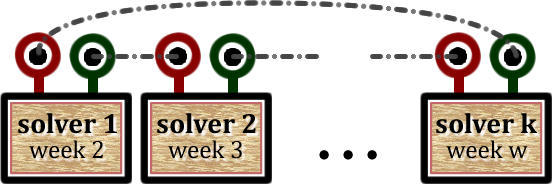
\includegraphics[width=0.45\linewidth]{golfers_ring.png}
	} %\hspace{0.1\linewidth}
	\subfloat[][]{%
		\label{subfig:golfers_bad_dic}
		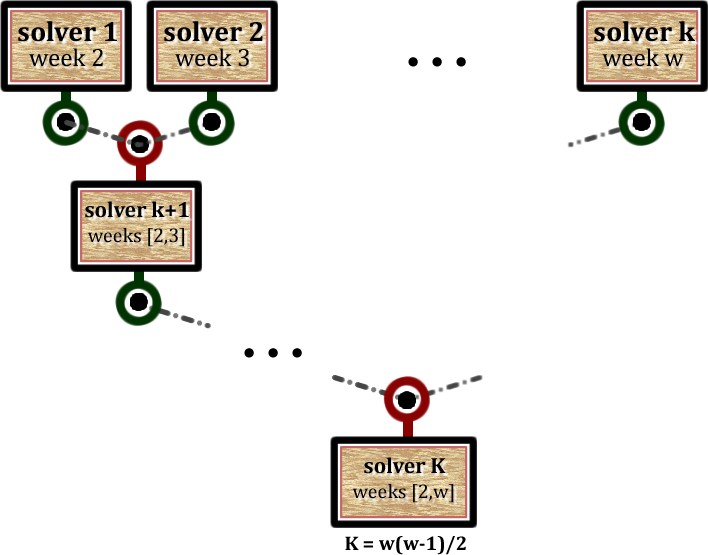
\includegraphics[width=0.45\linewidth]{golfers_dic.png}
	}
	\caption[]{Unsuccessful communication strategies to solve \SGP}
	\label{fig:golfers_bad}
\end{figure}

\separation

One last experiment using this benchmark was a \commstr{}, which applies a mechanism of cost descending acceleration, exchanging the current configuration between two solvers with different characteristics. Results show that this \commstr{} works pretty well for this problem.

For this strategy, new solvers were built reusing same \ms{} used for the \commstrs{} exposed before, and another different neighborhood \om{}: $V_{BP}(p)$, which given a configuration, returns the neighborhood $V\left(s\right)$ by swapping the culprit player chosen for all $p$ randomly selected weeks with other players in the same week. This new solver was called \textit{partial solver}, and it descends quicker the cost of its current solution at the beginning because its neighborhood generates less values, but the convergence is slower and yet not sure. It was combined with the solver used for the \commstrs{} exposed before. It was called \textit{full solver}, and converges in a stable way to the solution. So, the partial solver uses the same neighborhood function that the full solver, but parametrized in such a way that it builds neighbors only swapping players among two weeks. 

The idea of the \commstr{} is to communicate a configuration from the partial solver to the full solver. Here, the receiver solvers receive a configuration from a sender solver, and match it with their current configuration. Then it selects the configuration with the lowest global cost. This operation is coded using the \textit{minimum} operator $\poslop{m}$ in Algorithm~\ref{as:golfers_full}. This way, the full solver continues the search from a more promising place into de search space. After some iterations, is the full solver who sends its configuration to the partial solver. The partial solver takes this received configuration and starts its search from it and finds quickly a much better configuration to send to the full solver again. To force the partial solver to take the received configurations over its own, we use the \textit{not null} operator together with the \opch{} $C.M.$ (Algorithm~\ref{as:golfers_partial}). This process is repeated until a solution is found.

Figure~\ref{fig:solversgolfers} shows a full solver's run versus a partial solver's run. In this chart we can see that, at the beginning of the run, found configurations by the partial solver have costs significantly lower than those found by the full solver. \tet{At the 60-th millisecond} the full solver current configuration has cost 123, and the partial solver's one, 76. So for example, the communication at this time, can accelerate the process significantly.

\begin{figure}
\centering
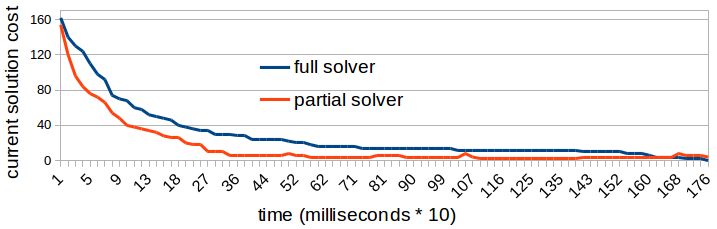
\includegraphics[width=\columnwidth]{graph.png} 
\caption{Partial solver vs. full solver (solving \sgp)}
\label{fig:solversgolfers}
\end{figure}

\begin{algorithm}
\dontprintsemicolon
\SetNoline
\SetKwProg{myproc}{\tet{\bf abstract solver}}{\tet{\bf begin}}{\tet{\bf end}}
\myproc{as\_full \;
	\tet{\bf computation} : $I, V, S_1, S_2, A$\;
	\tet{\bf communication} : $C.M.$\;}{%
	$I \poslop{\mapsto}$
	\whileinline{$\left(\textbf{\Iter} < K_1\right)$}{
		$V \poslop{\mapsto} \left[S_1 \poslopcond{\Sci \% K_1} S_1\right] \poslop{\mapsto} \left[C.M. \poslop{m} \llparenthesis A \rrparenthesis^d\right]$		
	}
}
\tet{\bf solver} \solverposl{full} \tet{\bf implements} as\_full\;
\algoindent \tet{\bf computation} : $I_{BP}, V_{BAS}, S_{first}, S_{rand}, A_{AI}$ \;
\algoindent \tet{\bf communication} : $CM_{last}$ \;
\caption{Full solver for \sgp}\label{as:golfers_full}
\end{algorithm}

\begin{algorithm}
\dontprintsemicolon
\SetNoline
\SetKwProg{myproc}{\tet{\bf abstract solver}}{\tet{\bf begin}}{\tet{\bf end}}
\myproc{as\_partial \;
	\tet{\bf computation} : $I, V, S_1, S_2, A$\;
	\tet{\bf communication} : $C.M.$\;}{
	$I \poslop{\mapsto}$
	\whileinline{$\left(\textbf{\Iter} < K_1\right)$}{
		$V \poslop{\mapsto} \left[S_1 \poslopcond{\Sci \% K_1} S_2\right] \poslop{\mapsto} \left[C.M. \poslop{\vee} \llparenthesis A \rrparenthesis^d\right]$		
	}
}
\tet{\bf solver} \solverposl{partial} \tet{\bf implements} as\_partial\;
\algoindent \tet{\bf computation} : $I_{BP}, V_{BP}(2), S_{first}, S_{rand}, A_{AI}$ \;
\algoindent \tet{\bf communication} : $CM_{last}$ \;
\caption{Partial \as{} for SGP}\label{as:golfers_partial}
\end{algorithm}

We also design different \commstrs, combining connected and unconnected solvers in different percentages, and applying two different \commopers: \oneTone{} and \oneTn.

This strategy produces some gain in terms of runtime as we can see in Tables~\ref{tab:golfers_v2_1N} and \ref{tab:golfers_v2_11} with respect to Table~\ref{tab:golfersB001}. It produces also more robust results in terms of runtime. The spread of results in iterations show higher variances, because there are included also results of partial solvers, which performs many times more iterations that the full solvers. The percentage of the receiver solvers that were able to find the solution before the others did, was significant (see Appendix~\ref{app:sgp}). That shows that the communication played an important role during the search, despite inter--process communication's overheads (reception, information interpretation, making decisions, etc).

The code for the \commstr{} of 100\% of communicating solvers is presented in Algorithm~\ref{comm:golfers_v2_100} and for 50\% of communicating solvers in Algorithm~\ref{comm:golfers_v2_50}. 

\begin{algorithm}[H]
\dontprintsemicolon
\SetNoline
$\left[\eqsolverposl{partial}\cdot A\right] \onetoone \left[\eqsolverposl{full}\cdot C.M.\right]20;$\;
$\left[\eqsolverposl{full}\cdot A\right] \onetoone \left[\eqsolverposl{partial}\cdot C.M.\right]20;$
\caption{Full-partial communication strategy 100\% communication}\label{comm:golfers_v2_100}
\end{algorithm}

\begin{algorithm}[H]
\dontprintsemicolon
\SetNoline
$\left[\eqsolverposl{partial}\cdot A\right] \onetoone \left[\eqsolverposl{full}\cdot C.M.\right]10;$\;
$\left[\eqsolverposl{full}\cdot A\right] \onetoone \left[\eqsolverposl{partial}\cdot C.M.\right]10;$\;
$\left[\eqsolverposl{first}\right]20;$\;
\caption{Full-partial communication strategy 100\% communication}\label{comm:golfers_v2_50}
\end{algorithm}

\begin{table}
\captionsetup{belowskip=6pt,aboveskip=6pt}
\centering 
\renewcommand{\arraystretch}{1}
\resizebox{\columnwidth}{!}{%
\begin{tabular}{p{1.5cm}|R{0.8cm}R{1cm}R{0.6cm}R{1.1cm}|R{0.8cm}R{1cm}R{0.6cm}R{1.1cm}|R{0.8cm}R{1cm}R{0.6cm}R{1.1cm}}
	\hline 	
	\multirow{2}{*}{\centering {\bf Instance}} & \multicolumn{4}{c|}{Comm. \oneTn} & \multicolumn{4}{c}{(Comm. \oneTn)/2} & \multicolumn{4}{c}{(Comm. \oneTn)/4}\\
	\cline{2-13}
	& T & T(sd) & It. & It.(sd) & T & T(sd) & It. & It.(sd) & T & T(sd) & It. & It.(sd) \\
	\hline
	%\hline
	5--3--7 & 0.14 & 0.08 & 102 & 53 & 0.14 & 0.07 & 97 & 73 & 0.12 & 0.08 & 175 & 162 \\
	8--4--7 & 0.30 & 0.13 & 101 & 24 & 0.22 & 0.06 & 92 & 29 & 0.22 & 0.06 & 88 & 45 \\
	9--4--8 & 0.55 & 0.15 & 125 & 20 & 0.53 & 0.14 & 107 & 20 & 0.40 & 0.14 & 101 & 70 \\
	\hline
\end{tabular}
}
\caption{Full-partial \commstr{} with communication \oneTn}
\label{tab:golfers_v2_1N}
\end{table}

\begin{table}
\captionsetup{belowskip=6pt,aboveskip=6pt}
\centering 
\renewcommand{\arraystretch}{1}
\resizebox{\columnwidth}{!}{%
\begin{tabular}{p{1.5cm}|R{0.8cm}R{1cm}R{0.6cm}R{1.1cm}|R{0.8cm}R{1cm}R{0.6cm}R{1.1cm}|R{0.8cm}R{1cm}R{0.6cm}R{1.1cm}}
	\hline 	
	\multirow{2}{*}{\centering {\bf Instance}} & \multicolumn{4}{c|}{Comm. \oneTone{} (100\%)} & \multicolumn{4}{c|}{Comm. \oneTone{} (50\%)} & \multicolumn{4}{c}{Comm. \oneTone{} (25\%)}\\
	\cline{2-13}
	& T & T(sd) & It. & It.(sd) & T & T(sd) & It. & It.(sd) & T & T(sd) & It. & It.(sd) \\
	\hline
	%\hline
	5--3--7 & 0.10 & 0.05 & 98 & 75 & \good{0.08} & 0.04 & 139 & 122 & 0.11 & 0.05 & 190 & 142 \\
	8--4--7 & \good{0.14} & 0.05 & 100 & 64 & 0.22 & 0.06 & 119 & 74 & 0.21 & 0.5 & 101 & 64 \\
	9--4--8 & 0.37 & 0.14 & 86 & 65 & \good{0.36} & 0.12 & 144 & 92 & 0.45 & 0.11 & 150 & 96 \\
	\hline
\end{tabular}
}
\caption{Full-partial \commstr{} with communication \oneTn}
\label{tab:golfers_v2_11}
\end{table}



%This confirms the intuition that parallel approach increases the probability of finding the solution within a more reasonable time (some tens of seconds), than with the sequential scheme \cite{Alon2011}. 
%The column labeled \textbf{\% success} in Table~\ref{tab:golfers_seq} indicates the percentage of solvers finding a solution before reaching a time--out (5 minutes). 
%presented in Table~\ref{tab:golfersB001}, column \textit{O.M. First Improvement} (without communication), and results with communication (Tables~\ref{tab:golfersB001comm100}, \ref{tab:golfersB001comm50} and \ref{tab:golfersB001comm25}). 

%\subsection{Analysis of results}
%
%
%
%
%\modified{Then we ran experiments to study \posl's behavior solving target problems in communicating scenarios. Some compositions of solvers set were taken into account:}
%\begin{inparaenum}[i.]
%	\item the structure of the communication (with/without communication or a mix), and
%	\item \modified{the used communication operator}.
%\end{inparaenum}

\section{Solving the \nqp}
\label{sec:nqueens}

\modified{In this section I present the performed study using \nqp{} (\NQP) as a benchmark.}

\subsection{Problem definition}

The \nqp{} (\NQP) asks how to place $N$ queens on a chess board so that none of them can hit any other in one move. \modified{This problem was introduced in 1848 by the chess player Max Bezzelas as the \textit{8-queen problem}, and years latter it was generalized as \textit{N-queen problem} by Franz Nauck. Since then many mathematicians, including Gauss, have worked on this problem. It finds a lot of applications, e.g., parallel memory storage schemes, traffic control, deadlock prevention, neural networks, constraint satisfaction problems, among others \cite{Bell2009}. Some studies suggest that the number of solution grows exponentially with the number of queens ($N$), but local search methods have been shown very good results for this problem \cite{Sosic1994}. For that reason we tested some communication strategies using \posl{}, to solve a problem relatively easy to solve using non communication strategies.}

\modified{The cost function for this benchmark was implemented in C++ based on the current implementation of {\it Adaptive Search}\footnote{It is based on the code from Daniel D\'{i}az available at \href{https://sourceforge.net/projects/adaptivesearch/}{https://sourceforge.net/projects/adaptivesearch/}}.}

\subsection{Experiment design Nr. 1}

To handle this problem, I reused some modules used for the \sgp: the \textit{Selection} and \textit{Acceptance} modules. The new module is: 

\begin{enumerate}
	\item Neighborhood module:
	\subitem $V_{AS}$: Defines the neighborhood $V\left(s\right)$ swapping the variable which contributes the most to the cost with other.
\end{enumerate}

\modified{Fors this problem I used a simple \as{} showing good results with no communication, based on the idea introduced in the section \ref{sec:golfers}, using the \om{} $S_{rand}$ to scape from local minima. The \as{} is presented in Algorithm~\ref{as:nq}.}

\begin{algorithm}[H]
\dontprintsemicolon
\SetNoline
\SetKwProg{myproc}{\tet{\bf abstract solver}}{\tet{\bf begin}}{\tet{\bf end}}
\myproc{as\_eager \tcp*{{\sc Itr} $\rightarrow$ number of iterations}
	\tet{\bf computation} : $I, V, S_1, S_2, A$\tcp*{{\sc Sci} $\rightarrow$ number of iterations with the same cost}}{
	$I \poslop{\mapsto}$
		\whileinline{$\left(\textbf{\Iter < } K_1\right)$}{$ V \poslop{\mapsto} \left[S_1 \poslopcond{\Sci < K_2} S_2\right] \poslop{\mapsto} A$}	
}
\caption{\As{} for \NQP}\label{as:nq}
\end{algorithm}

Using solvers implementing this \as{} we create communicating solvers to compare their performance with the non communicating strategies. The shared information is the current configuration. Algorithms~\ref{as:nq_sender}~and~\ref{as:nq_receiver} show that the communication is performed while selecting a new configuration for the next iteration. We design different communication strategies. Either I execute a full connected solvers set, or a tuned combination of connected and unconnected solvers. Between connected solvers, I have applied two different connections operations: connecting each sender solver with one receiver solver ({\it 1~to~1}), or connecting each sender solver with all receiver solvers ({\it 1~to~N}).

\begin{algorithm}[H]
\dontprintsemicolon
\SetNoline
\SetKwProg{myproc}{\tet{\bf abstract solver}}{\tet{\bf begin}}{\tet{\bf end}}
\myproc{as\_eager\_sender \tcp*{{\sc Itr} $\rightarrow$ number of iterations}
	\tet{\bf computation} : $I, V, S_1, S_2, A$\tcp*{{\sc Sci} $\rightarrow$ number of iterations with the same cost}}{
	$I \poslop{\mapsto}$
		\whileinline{$\left(\textbf{\Iter < } K_1\right)$}{$ V \poslop{\mapsto} \left[\llparenthesis S_1 \rrparenthesis^o \poslopcond{\Sci < K_2} S_2\right] \poslop{\mapsto} A$}	
}
\caption{\As{} for \NQP{} (sender)}\label{as:nq_sender}
\end{algorithm}

\begin{algorithm}[H]
\dontprintsemicolon
\SetNoline
\SetKwProg{myproc}{\tet{\bf abstract solver}}{\tet{\bf begin}}{\tet{\bf end}}
\myproc{as\_eager\_receiver \tcp*{{\sc Itr} $\rightarrow$ number of iterations}
	\tet{\bf computation} : $I, V, S_1, S_2, A$\tcp*{{\sc Sci} $\rightarrow$ number of iterations with the same cost}
	\tet{\bf communication} : $C.M.$\;}{%
	$I \poslop{\mapsto}$\\
		\While{$\left(\textbf{\Iter < } K_1\right)$}{$ V \poslop{\mapsto} \left[ \left[S_1 \poslopcond{\Iter \% K_2} \left[S_1 \poslop{m} C.M. \right]\right] \poslopcond{\Sci < K_3} S_2\right] \poslop{\mapsto} A$}	
}
\caption{\As{} for \NQP{} (receiver)}\label{as:nq_receiver}
\end{algorithm}

\subsection{Results analysis of experiment Nr. 1}

\modified{I use directly the neighborhood module $V_{AS}$ based on the {\it Adaptive Search} algorithm, and the selection module $S_{First}$ which selects the first configuration inside the neighborhood improving the current cost, to create solvers, and studying communicating and non communicating strategies.}

\begin{table}[h]
\centering 
\renewcommand{\arraystretch}{1}
\resizebox{\columnwidth}{!}{%
\begin{tabular}{p{1.3cm}|R{1.3cm}R{1.3cm}R{1.3cm}R{1.3cm}|R{1.3cm}R{1.3cm}R{1.3cm}R{1.3cm}}
	\hline %\noalign{\smallskip}	
	\multirow{2}{*}{\footnotesize{\centering {\bf Instance}}} & \multicolumn{4}{c|}{\bf Sequential (1 core)} & \multicolumn{4}{c}{\bf No Comm. (40 cores)} \\
	\cline{2-9}
	& T & T(sd) & It. & It.(sd) & T & T(sd) & It. & It.(sd) \\	
	\hline
	2000 & 6.20 & 0.12 & 947 & 21 & 6.15 & 0.20 & 952 & 20 \\
	3000 & 14.19 & 0.21 & 1,415 & 22 & 14.06 & 0.33 & 1,413 & 25 \\
	4000 & 25.63 & 0.36 & 1,900 & 28 & 25.46 & 0.51 & 1,898 & 34 \\
	5000 & 41.37 & 0.44 & 2,367 & 26 & 40.57 & 0.91 & 2,377 & 32 \\
	6000 & 60.42 & 0.52 & 2,837 & 31 & 60.10 & 0.70 & 2,849 & 43 \\
	\hline
\end{tabular}
}
\caption{Results for \NQP{} (no communication)}\label{tab:nqueens_seq}
\end{table}

\begin{table}[h]
\centering 
\renewcommand{\arraystretch}{1}
\newcommand{\cwnq}{1.1cm}
\resizebox{\columnwidth}{!}{%
\begin{tabular}{p{1.3cm}|R{\cwnq}R{\cwnq}R{\cwnq}R{\cwnq}|R{\cwnq}R{\cwnq}R{\cwnq}R{\cwnq}|R{\cwnq}R{\cwnq}R{\cwnq}R{\cwnq}}
	\hline %\noalign{\smallskip}	
	\multirow{2}{*}{\footnotesize{\centering {\bf Instance}}} & \multicolumn{4}{c|}{\bf 25\% Comm.} & \multicolumn{4}{c|}{\bf 50\% Comm.} &  \multicolumn{4}{c}{\bf All Comm.}\\
	\cline{2-13}
	& T & T(sd) & It. & It.(sd) & T & T(sd) & It. & It.(sd) & T & T(sd) & It. & It.(sd) \\	
	\hline
	2000 & 6.05 & 0.25 &  934 & 36 & 6.01 & 0.19 & 920 & 41 & 5.92 & 0.17 & 885 & 49\\ 
	3000 & 13.89 & 0.28 & 1,387 & 48 & 13.91 & 0.30 & 1,368 & 51 & 13.67 & 0.39 & 1,346 & 40 \\
	4000 & 25.26 & 0.63 & 1,868 & 43 & 25.14 & 0.50 & 1,855 & 50 & 25.11 & 0.39 & 1,834 & 58 \\
	5000 & 40.38 & 0.93 & 2,338 & 71 & 40.33 & 0.66 & 2,312 & 69 & 39.62 & 1.07 & 2,287 & 44 \\
	6000 & 59.28 & 1.34 & 2,794 & 78 & 58.97 & 1.19 & 2,775 & 67 & 58.97 & 1.38 & 2,729 & 78 \\	
	\hline
\end{tabular}
}
\caption{Results for \NQP{} (40 cores, communication 1~to~1)}\label{tab:nqueens_1to1}
\end{table}

\begin{table}[h]
\centering 
\renewcommand{\arraystretch}{1}
\newcommand{\cwnq}{1.1cm}
\resizebox{\columnwidth}{!}{%
\begin{tabular}{p{1.3cm}|R{\cwnq}R{\cwnq}R{\cwnq}R{\cwnq}|R{\cwnq}R{\cwnq}R{\cwnq}R{\cwnq}|R{\cwnq}R{\cwnq}R{\cwnq}R{\cwnq}}
	\hline %\noalign{\smallskip}	
	\multirow{2}{*}{\footnotesize{\centering {\bf Instance}}} & \multicolumn{4}{c|}{\bf 25\% Comm.} & \multicolumn{4}{c|}{\bf 50\% Comm.} &  \multicolumn{4}{c}{\bf All Comm.}\\
	\cline{2-13}
	& T & T(sd) & It. & It.(sd) & T & T(sd) & It. & It.(sd) & T & T(sd) & It. & It.(sd) \\	
	\hline
	2000 & 6.07 & 0.15 & 925 & 41 & 5.98 & 0.19 & 915 & 41 & 6.01 & 0.19 & 887 & 57 \\
	3000 & 13.97 & 0.34 & 1,402 & 49 & 13.96 & 0.31 & 1,386 & 52 & 13.79 & 0.32 & 1,365 & 65 \\
	4000 & 25.30 & 0.57 & 1,867 & 52 & 25.29 & 0.42 & 1,851 & 66 & 25.17 & 0.47 & 1,838 & 65 \\
	5000 & 40.45 & 0.80 & 2,338 & 80 & 40.37 & 0.56 & 2,312 & 56 & 39.88 & 0.71 & 2,291 & 51 \\
	6000 & 59.77 & 1.50 & 2,824 & 49 & 59.53 & 0.98 & 2,773 & 69 & 59.16 & 1.37 & 2,773 & 57 \\	
	\hline
\end{tabular}
}
\caption{Results for \NQP{} (40 cores, communication 1~to~N)}\label{tab:nqueens_1toN}
\end{table}

\modified{\posl{}, as it can be seen} in Tables~\ref{tab:nqueens_1to1} and~\ref{tab:nqueens_1toN}, works very well without communication, for instances relatively big. This confirms once again the success of the \om{} $V_{AS}$ based on {\it Adaptive Search} algorithm to solve these kind of problems. That is the reason why the parallel approach does not outperforms significantly the sequential one, as we can see in Table~\ref{tab:nqueens_seq}. However, the communication improve the non communicating results in terms of runtime and iterations, but this improvement is not significant. In contrast to \SGP, \posl{} does not get trapped so often into local minima during the resolution of \NQP{}. For that reason, the shared information, once received and accepted by the receivers solvers, does not improves largely the current cost.

\modified{We can see the improvement with respect to the percentage of} communicating solvers in Figure~\ref{fig:results_nq}. The bigger the instance is, the more significant the observed improvement is. This phenomenon suggests that a deeper study and an efficient implementation can make the communication playing a more significant role in the solution process. For that reason, I decided to design another experiment to try to improve the results using communicating strategies using \posl.

\pgfplotsset{
	myStyle/.style={grid=major,font=\Large}, ylabel= Communication rate,
	xlabel=Number of cores,
	legend style={at={(0.7,0.9)},
	anchor=north}
}

\begin{figure}
\centering
\begin{tikzpicture} [scale=0.7]
\begin{groupplot}[
group style={
	group name=my plots,
	group size=1 by 5,
	xlabels at=edge bottom,
	xticklabels at=edge bottom,		
	ylabels at=edge left,
	yticklabels at=edge left,
	vertical sep=0pt
},
legend style={at={(0.32,0.40)},anchor=north, legend columns=2},
footnotesize,
width=14cm,
height=4.5cm,
xlabel=\% of communicating solvers,
ylabel= \empty,
xmin=-5,
xmax=105,
ymin=0,	
ymax=30,
ytick={0,10,...,20},
xtick={0,25,50,100},
tickpos=left,
ytick align=outside,
xtick align=outside]

\nextgroupplot %2000
[ymin=5.6, ymax=6.2, ytick={5.7,5.8,5.9,6.0,6.1,6.2}, cycle list ={{red, mark options={fill=red,scale=0.8},mark=*}, {blue, mark options={fill=blue,scale=0.8},mark=*}, {green, mark options={fill=green,scale=0.8},mark=*}, {orange, mark options={fill=orange,scale=0.8},mark=x}}]
\addlegendentry{1 to 1}
\addplot coordinates{(0,6.15) (25,6.05) (50,6.01) (100,5.92)};
\addlegendentry{1 to N}
\addplot coordinates{(0,6.15) (25,6.07) (50,5.98) (100,6.01)};

\nextgroupplot %3000
[ymin=13.5, ymax=14.1, ytick={13.6,13.7,13.8,13.9,14.0,14.1}, cycle list ={{red, mark options={fill=red,scale=0.8},mark=*}, {blue, mark options={fill=blue,scale=0.8},mark=*}, {green, mark options={fill=green,scale=0.8},mark=*}, {orange, mark options={fill=orange,scale=0.8},mark=x}}]
\addplot coordinates{(0,14.06) (25,13.89) (50,13.91) (100,13.67)};
\addplot coordinates{(0,14.06) (25,13.97) (50,13.96) (100,13.79)};

\nextgroupplot %4000
[ymin=24.9, ymax=25.5, ytick={25.0,25.1,25.2,25.3,25.4,25.5}, cycle list ={{red, mark options={fill=red,scale=0.8},mark=*}, {blue, mark options={fill=blue,scale=0.8},mark=*}, {green, mark options={fill=green,scale=0.8},mark=*}, {orange, mark options={fill=orange,scale=0.8},mark=x}}, ylabel= runtime (secs)]
\addplot coordinates{(0,25.46) (25,25.25) (50,25.14) (100,25.11)};
\addplot coordinates{(0,25.46) (25,25.30) (50,25.29) (100,25.17)};

\nextgroupplot %5000
[ymin=39.5, ymax=40.7, ytick={39.6,39.8,40.0,40.2,40.4,40.6}, cycle list ={{red, mark options={fill=red,scale=0.8},mark=*}, {blue, mark options={fill=blue,scale=0.8},mark=*}, {green, mark options={fill=green,scale=0.8},mark=*}, {orange, mark options={fill=orange,scale=0.8},mark=x}}]
\addplot coordinates{(0,40.57) (25,40.38) (50,40.33) (100,39.62)};
\addplot coordinates{(0,40.57) (25,40.45) (50,40.37) (100,39.88)};

\nextgroupplot %6000
[ymin=58.8, ymax=60.4, ytick={58.8,59.1,59.4,59.7,60.0,60.3}, cycle list ={{red, mark options={fill=red,scale=0.8},mark=*}, {blue, mark options={fill=blue,scale=0.8},mark=*}, {green, mark options={fill=green,scale=0.8},mark=*}, {orange, mark options={fill=orange,scale=0.8},mark=x}}]
\addplot coordinates{(0,60.10) (25,59.28) (50,58.97) (100,58.97)};
\addplot coordinates{(0,60.10) (25,59.77) (50,59.53) (100,59.16)};
		
\end{groupplot}
\end{tikzpicture}
\caption[]{Runtime means of instances \\2000-, 3000-, 4000-, 5000- and 6000-queens}
\label{fig:results_nq}
\end{figure}

\subsection{Experiment design Nr. 2}

\modified{The strategy of work sub-division proposed in the previews section} with \sgp{} seemed interesting to me and I did not want to give up on it. So I tried to apply it to \nqp. 

\modified{In some experimental runs, I launched some {\it partial} solvers (i.e., solvers only performing permutations between variables into certain range)}, together with a {\it full} solver (i.e., a solver working with the entire configuration). I used the instance \textit{4000-queens} as test and I built the following solvers:
\begin{enumerate}
\item Solver $S_1$ only permuting the first 1000 variables
\item Solver $S_2$ only permuting the first 2000 variables
\item Solver $S_3$ only permuting the first 3000 variables
\item Solver $S_4$ a {\it full} solver.
\end{enumerate}

\modified{Obviously, } the first three solvers were not able to find a solution to the problem, but at the beginning of runs, it was possible to observe that these solvers were able to obtain configurations with costs considerably lower with respect to the {\it full} solver $S_4$. For that reason I put in practice the idea of connecting {\it partial} solvers together with {\it full} solvers. This way, the search process can be accelerated at the beginning.

\modified{Before designing} the solution strategy (\as) many experiments were launched to select: \begin{inparaenum} \item The number of sub-divisions of the configuration, i.e., how many {\it partial} solvers works in different sections of the configuration. They are connected to the {\it full} solver. \item The size of the section where the {\it partial} solvers work in. \end{inparaenum} 

\modified{After many runs} of these experiments, it was decided to work with two {\it partial} sender solvers (implementing the \as{} in Algorithm~\ref{as:nq_ex6_sender}). In this algorithm $a$ and $b$ are parameters of the module $V_{[a,b]}$ used in the {\it partial} solvers. They represent the variables defining the range of the configuration where the {\it partial} solver works. They were chosen such that $b-a = \tfrac{n}{4}$ These solvers send their configurations to the {\it full} solver that implements the \as{} in Algorithm~\ref{as:nq_ex6_receiver}.

\begin{algorithm}[H]
\dontprintsemicolon
\SetNoline
\SetKwProg{myproc}{\tet{\bf abstract solver}}{\tet{\bf begin}}{\tet{\bf end}}
\myproc{as\_partial\_sender \tcp*{{\sc Itr} $\rightarrow$ number of iterations}
	\tet{\bf computation} : $I, V_{[a,b]}, S, A$\tcp*{{\sc Sci} $\rightarrow$ number of iterations with the same cost}}{
	\While{$\left(\textbf{\Iter < } K_1\right)$}{
	$I \poslop{\mapsto}$
		\whileinline{$\left(\textbf{\Iter \% } K_2 || \textbf{ \Sci < } K_3\right)$}{$\left[V_{[a,b]} \poslop{\mapsto} S \poslop{\mapsto} \left[\llparenthesis A \rrparenthesis^o \poslopcond{\Iter \% K_4} A\right]\right] $}
	}	
}
\caption{\As{} for \NQP{} (partial solver sender)}\label{as:nq_ex6_sender}
\end{algorithm}

\begin{algorithm}[H]
\dontprintsemicolon
\SetNoline
\SetKwProg{myproc}{\tet{\bf abstract solver}}{\tet{\bf begin}}{\tet{\bf end}}
\myproc{as\_full\_receiver \tcp*{{\sc Itr} $\rightarrow$ number of iterations}
	\tet{\bf computation} : $I, V, S, A$\tcp*{{\sc Sci} $\rightarrow$ number of iterations with the same cost}
	\tet{\bf communication} : $C.M.$\;}{%
	$I \poslop{\mapsto}$\\
		\While{$\left(\textbf{\Iter < } K_1\right)$}{$\left[ V \poslop{\mapsto} S \poslop{\mapsto} \left[A \poslopcond{\Iter \% K_2} \left[A \poslop{m} C.M. \right]\right] \right]$}	
}
\caption{\As{} for \NQP{} (full solver receiver)}\label{as:nq_ex6_receiver}
\end{algorithm}

\subsection{Results analysis of experiment Nr. 2}

\modified{Results in Table~\ref{tab:nqueens_dic}} show that this strategy is effective to solve the \nqp{} improving the runtimes already obtained in the previews experiment. In the resolution of this problem, the improvement rate of the current configuration cost is very slow (yet stable). The \textit{partial} solvers work only on a section of the configuration, and for that reason, they are able to obtain configuration with costs considerably lower than the obtained by the {\it full} solver more quickly. This characteristic is taken into account: \textit{partial} solvers send their obtained configurations to the \textit{full} solvers. By doing this, the improvement rate of the current configuration can be accelerated at the beginning of the search.

\begin{table}[h]
\centering 
\renewcommand{\arraystretch}{1}
\begin{tabular}{p{1.5cm}|R{1.5cm}R{1.5cm}R{1.5cm}R{1.5cm}}
	\hline 
	{\bf Instance} & T & T(sd) & It. & It.(sd) \\	
	\hline
	2000 & \good{\bf 5.11} & 0.83 & \good{\bf 841} & 37 \\
	3000 & \good{\bf 11.55} & 1.96 & \good{\bf 1,275} & 67 \\
	4000 & \good{\bf 21.27} & 3.76 & \good{\bf 1,656} & 108 \\
	5000 & \good{\bf 34.77} & 4.99 & \good{\bf 2,082} & 108 \\
	6000 & \good{\bf 51.72} & 5.73 & \good{\bf 2,501} & 176 \\	
	\hline
\end{tabular}
\caption{Results for \NQP{} (40 cores, communication partial-full solvers)}\label{tab:nqueens_dic}
\end{table}

\section{Solving the \carrp}
\label{sec:costas}

In this section I present the performed study using \carrp{} (\CARRP) as a benchmark. This time, a simple communication strategy, in which the information to communicate between solvers is the current configuration was tested, showing good results.

\subsection{Problem definition}

The \carrp{} (\CARRP) consists in finding a \textit{costas array}, which is an $n\times n$ grid containing $n$ marks such that there is exactly one mark per row and per column and the $n(n-1)/2$ vectors joining each couple of marks are all different. This is a very complex problem that finds useful application in some fields like sonar and radar engineering. It also presents an interesting characteristic: although the search space grows factorially, from order 17 the number of solutions drastically decreases~\cite{Drakakis2006}.

The cost function for this benchmark was implemented in C++ based on the current implementation of {\it Adaptive Search}\footnote{It is based on the code from Daniel D\'{i}az available at \href{https://sourceforge.net/projects/adaptivesearch/}{https://sourceforge.net/projects/adaptivesearch/}}.

\subsection{Experiment design and results}

To handle this problem, I have reused all modules used for solving the \nqp. First attempts to solve this problems were using the same strategies (\ass) used to solve the \sgp{} and \nqp, without success: \posl{} was not able to solve instances larger than $n = 8$ in a reasonable amount of time (seconds). After many unsuccessful attempts to find the rights parameter of \textit{maximum number of restarts}, \textit{maximum number of iterations}, and \textit{maximum number of iterations with the same cost}, I decided to implement the mechanism used by Daniel D\'iaz in the current implementation of {\it Adaptive Search} to escape from local minima: I have added a {\it Reset} \om{} $R_{AS}$ based on the abstract \om{} $R$.

The basic solver I use to solve this problem is presented in Algorithm~\ref{as:costas}, and I take it as a base to build all the different communication strategies. Basically, it is a classical local search iteration, where instead of performing restarts, it performs resets. After a deep analysis of this implementation and results of some runs, I decided to use $K_1 = 24000$ (maximum number of iterations) big enough to solve the chosen instance $n = 17$; and $K_2 = 3$ (the number of iteration before performing the next \textit{reset}).

\begin{algorithm}[H]
\dontprintsemicolon
\SetNoline
\SetKwProg{myproc}{\tet{\bf abstract solver}}{\tet{\bf begin}}{\tet{\bf end}}
\myproc{as\_hard \tcp*{{\sc Itr} $\rightarrow$ number of iterations}
	\tet{\bf computation} : $I, R, V, S, A$\;}{ %\tcp*{{\sc Sci} $\rightarrow$ number of iterations with the same cost}}{%
	$I \poslop{\mapsto}$
	\whileinline{$\left(\textbf{\Iter < } K_1\right)$}{
		$R \poslop{\mapsto}$ % \left[\circlearrowleft (\text{\Iter}\% K_2) \left\{ M_V \longmapsto M_{\hat{S}} \longmapsto M_D\right\}\right]$\;
		\whileinline{$\left(\textbf{\Iter \% } K_2\right)$}{$\left[V \poslop{\mapsto} S \poslop{\mapsto} A\right]$}
	}
}
\tet{\bf solver} \solverposl{single} \tet{\bf implements} as\_hard\;
\algoindent \tet{\bf computation} : $I_{perm},  R_{AS}, V_{AS}, S_{first}, A_{AI}$ \;
%\tet{\bf connection}: $CM_{last}$\;
\caption{Reset-based \as{} for \CARRP}\label{as:costas}
\end{algorithm}

I present in Table~\ref{tab:costas19} results of launching {\it solver sets} to solve each instance of \carrp{} 19 sequentially and in parallel without communication. Runtimes and iteration means showed in this confirm once again the success of the parallel approach. 

\begin{table}[h]
\captionsetup{belowskip=6pt,aboveskip=6pt}
\centering
\renewcommand{\arraystretch}{1}
\begin{tabular}{p{3.5cm}|R{1.5cm}R{1cm}R{1.7cm}R{1.7cm}R{2cm}}
	\hline
	{\bf STRATEGY} & T & T(ds) & It. & It.(sd) & \% success\\
	\hline
	%\hline
	Sequential (1 core) & 132.73 & 80.32 & 2,332,088 & 1,424,757 & 40.00\\
	Parallel (40 cores) & 25.51 & 15.75 & 231,262 & 143,789 & 100.00\\
	\hline
\end{tabular}
\caption{\carr{} 19: no communication}
\label{tab:costas19}
\end{table}

\separation

In order to improve results, a simple communication strategy was applied: communicating the current configuration to other solvers. To do so, we insert a \textit{sending output} operator to the \as{} in Algorithm~\ref{as:costas}. This results in the sender solver presented in Algorithm~\ref{as:costas_sender}. %\tet{et le receiver??? Flo: c'est l'algo 4}

\begin{algorithm}[H]
\dontprintsemicolon
\SetNoline
\SetKwProg{myproc}{\tet{\bf abstract solver}}{\tet{\bf begin}}{\tet{\bf end}}
\myproc{as\_hard\_sen \; %\hspace{3pt}
	\tet{\bf computation} : $I, R, V, S, A$\;}{
	$I \poslop{\mapsto}$
	\whileinline{$\left(\textbf{\Iter} < K_1\right)$}{
		$T \poslop{\mapsto}$
		\whileinline{$\left(\textbf{\Iter \% } K_2\right)$}{$\left[V \poslop{\mapsto} S \poslop{\mapsto} \llparenthesis A \rrparenthesis^d\right]$}
	}
}
\tet{\bf solver} \solverposl{sender} \tet{\bf implements} as\_hard\_sen\;
\algoindent \tet{\bf computation} : $I_{perm}, R_{AS}, V_{AS}, S_{first}, A_{AI}$ \;
%\tet{\bf connection}: $CM_{last}$\;
\caption{Sender solver for \CARRP}\label{as:costas_sender}
\end{algorithm}

Studying some runs of \posl{} for solving \CARRP{}, it was observed that the cost of the current configuration of the first solver finding a solution. This cost describes an oscillatory descent due to the repeated resets. For that reason, it was decided to apply a simple \commstr{} that shares the current configuration while applying the acceptance criterion: its goal is to  accelerate the cost descent. To do so, a \opch{} using a \textit{minimum} operator $\poslop{m}$ together with the abstract \om{} $A$ was inserted, as shown in Algorithm~\ref{as:costas_receiver_a}.

One of the main purpose of this study is to explore different communication strategies. We have then implemented and tested different variations of the strategy exposed above by combining two communication operators (\oneTone{} and \oneTn) and different percentages of communicating solvers.
For this problem, it was study also the behavior of the communication performed at two different moments: while applying the acceptance criteria (Algorithm~\ref{as:costas_receiver_a}), and while performing a {\it reset} (Algorithm~\ref{as:costas_receiver_b}).

\begin{algorithm}[H]
\dontprintsemicolon
\SetNoline
\SetKwProg{myproc}{\tet{\bf abstract solver}}{\tet{\bf begin}}{\tet{\bf end}}
\myproc{as\_hard\_receiver\_a \tcp*{{\sc Itr} $\rightarrow$ number of iterations}
	\tet{\bf computation} : $I, T, V, S, A$ \; %\hspace{3pt}
	\tet{\bf communication} : $C.M.$\;}{ 
	$I \poslop{\mapsto}$
	\whileinline{$\left(\textbf{\Iter} < K_1\right)$}{
		$T \poslop{\mapsto}$
		\whileinline{$\left(\textbf{\Iter \% } K_2\right)$}{$\left[V \poslop{\mapsto} S \poslop{\mapsto} \left[A\poslop{m}C.M.\right]\right]$}
	}
}
\tet{\bf solver} \solverposl{receiverA} \tet{\bf implements} as\_hard\_receiver\_a\;
\algoindent\tet{\bf computation} : $I_{perm}, R_{AS}, V_{AS}, S_{first}, A_{AI}$ \; 
\algoindent\tet{\bf communication}: $CM_{last}$\;
\caption{Receiver solver for \CARRP{} (variant A)}\label{as:costas_receiver_a}
\end{algorithm}

\begin{algorithm}[H]
\dontprintsemicolon
\SetNoline
\SetKwProg{myproc}{\tet{\bf abstract solver}}{\tet{\bf begin}}{\tet{\bf end}}
\myproc{as\_hard\_receiver\_b \tcp*{{\sc Itr} $\rightarrow$ number of iterations}
	\tet{\bf computation} : $I, R, V, S, A$\; %\tcp*{{\sc Sci} $\rightarrow$ number of iterations with the same cost}
	\tet{\bf communication} : $C.M.$\;}{%
	$I \poslop{\mapsto}$
	\whileinline{$\left(\textbf{\Iter < } K_1\right)$}{
		$\left[R \poslop{m} C.M.\right] \poslop{\mapsto}$
		\whileinline{$\left(\textbf{\Iter \% } K_2\right)$}{$\left[V \poslop{\mapsto} S \poslop{\mapsto} A\right]$}
	}
}
\tet{\bf solver} \solverposl{receiverB} \tet{\bf implements} as\_hard\_receiver\_b\;
\algoindent\tet{\bf computation} : $I_{perm}, R_{AS}, V_{AS}, S_{first}, A_{AI}$ \; 
\algoindent\tet{\bf connection}: $CM_{last}$\;
\caption{Receiver solver for \CARRP{} (variant B)}\label{as:costas_receiver_b}
\end{algorithm}

The instantiation for the receiver solvers instantiates the abstract \opch{} $C.M.$ with the concrete \opch{} $CM_{last}$, which takes into account the last received configuration when it is running.

\begin{table}
\centering 
\renewcommand{\arraystretch}{1}
\resizebox{\columnwidth}{!}{%
\begin{tabular}{p{2.5cm}|R{1.1cm}R{1cm}R{1.3cm}R{1.3cm}|R{1cm}R{1cm}R{1.3cm}R{1.3cm}}
	\hline
	\multirow{3}{*}{\footnotesize{\centering {\bf STRATEGY}}} & \multicolumn{4}{c}{100\% COMM} & \multicolumn{4}{c}{50\% COMM} \\
	\cline{2-9}
	& T & T(sd) & It. & It.(sd) & T & T(sd) & It. & It.(sd)\\
	\hline
	Str A: 1 to 1 & 11.60 & 9.17 & 84,159 & 68,958 & 16.78 & 13.43 & 148,222 & 121,688 \\
	Str A: 1 to N & \good{10.83} & 8.72 & 79,551 & 63,785 & 13.03 & 13.46 & 106,826 & 120,894 \\	
	Str B: 1 to 1 & 14.84 & 13.54 & 119,635 & 112,085 & 14.51 & 13.88 & 125,982 & 123,261 \\
	Str B: 1 to N & 22.99 & 23.82 & 199,930 & 207,851 & 16.62 & 15.16 & 138,840 & 116,858 \\
	\hline
\end{tabular}
}
\caption{\carr{} 19: with communication}
\label{tab:costas19comm}
\end{table}

Table~\ref{tab:costas19comm} shows that \sosets{} executing the strategy {\it A} (receiving the configuration at the time of applying the acceptance criteria) is more effective. The reason is that the others, interfere with the proper performance of the {\it reset}, that is a very important step in the algorithm. This step can be performed on three different ways:
\begin{enumerate}
\item Trying to shift left/right all sub-vectors starting or ending by the variable which contributes the most to the cost, and selecting the configuration with the lowest cost.
\item Trying to add a constant (circularly) to each element in the configuration.
\item Trying to shift left from the beginning to some culprit variable (i.e., a variable contributing to the cost).
\end{enumerate}
Then, one of these 3 generated configuration has the sabe probability of being selected, to be the result of the \textit{reset} step. In that sense, some different \textit{resets} can be performed for the same configuration. Here is when the communication play its important role: receiver and sender solvers apply different \textit{reset} in the same configuration, and results showed the efficacy of this communication strategy.
 
Analyzing the whole information obtained during the experiments, we can observe that the percentage of communicating solvers finding the solution thanks to the received information was high. That shows that the communicated information was very helpful during the search process. 
With the simplicity of the operator-based language provided by \posl{}, we were able to find a simple \commstr{} to obtain better results than applying sequential and parallel independent multi-walk approaches. As expected, the best strategy was based on 100\% of communication and a \oneTn{} communication, because this strategy allows to communicate a promising place inside the search space to a maximum of solvers, helping the decisive intensification process.
%(a good compromise between local computation and data exchange/a fully based communication/ etc)
Algorithm~\ref{comm:costas1001N} shows the code of this \commstr{}, where  20 is used as  \textit{syntactic sugar} to declare easily a list of 20 solvers of each type (20 senders and 20 receivers). Using the \oneTn{} operator $\oneton$ each sender solver sends information to every receiver solver. 

\begin{algorithm}
\dontprintsemicolon
\SetNoline
$\left[\eqsolverposl{sender}\cdot A(20)\right] \oneton \left[\eqsolverposl{receiverA}\cdot C.M.(20)\right];$
\caption{Communication strategy \oneTn{} 100\% for \CARRP}\label{comm:costas1001N}
\end{algorithm}

Table~\ref{tab:costas19comm} shows also high values of standard deviation. This is not surprising, due to the highly random nature of the neighborhood function and the selecting criterion, as well as the execution of many resets during the search process.




%\begin{algorithm}[H]
%\dontprintsemicolon
%\SetNoline
%\SetKwProg{myproc}{\tet{\bf abstract solver}}{\tet{\bf begin}}{\tet{\bf end}}
%\myproc{as\_hard\_receiver\_a \tcp*{{\sc Itr} $\rightarrow$ number of iterations}
%	\tet{\bf computation} : $I, R, V, S, A$\; %\tcp*{{\sc Sci} $\rightarrow$ number of iterations with the same cost}
%	\tet{\bf communication} : $C.M.$\;}{%
%	$I \poslop{\mapsto}$\\
%	\While{$\left(\textbf{\Iter < } K_1\right)$}{
%		$R \poslop{\mapsto}$
%		\whileinline{$\left(\textbf{\Iter \% } K_2\right)$}{$\left[V \poslop{\mapsto} S \poslop{\mapsto} \left[A \poslop{m} C.M.\right]\right]$}
%	}
%}
%\caption{Reset-based \as{} for \CARRP{} (receiver, variant A)}\label{as:costas_receiver_a}
%\end{algorithm}
%
%
%\begin{algorithm}[H]
%\dontprintsemicolon
%\SetNoline
%\SetKwProg{myproc}{\tet{\bf abstract solver}}{\tet{\bf begin}}{\tet{\bf end}}
%\myproc{as\_hard\_receiver\_c \tcp*{{\sc Itr} $\rightarrow$ number of iterations}
%	\tet{\bf computation} : $I, R, V, S, A$\; %\tcp*{{\sc Sci} $\rightarrow$ number of iterations with the same cost}
%	\tet{\bf communication} : $C.M.$\;}{%
%	$I \poslop{\mapsto}$\\
%	\While{$\left(\textbf{\Iter < } K_1\right)$}{
%		$\left[R \poslop{m} C.M.\right] \poslop{\mapsto}$
%		\whileinline{$\left(\textbf{\Iter \% } K_2\right)$}{$\left[V \poslop{\mapsto} S \poslop{\mapsto} A\right]$}
%	}
%}
%\caption{Reset-based \as{} for \CARRP{} (receiver, variant C)}\label{as:costas_receiver_c}
%\end{algorithm}



\section{Solving the \grp}
\label{sec:golomb}

In this section the performed study using \grp{} (\GRP) as a benchmark, is presented. Using this benchmark, a different communication strategy was tested: we communicate the current configuration in order to avoid its neighborhood, i.e., a {\it tabu} configuration.

\subsection{Problem definition}

The \grp{} (\GRP) problem consists in finding an ordered vector of $n$ distinct non-negative integers, called \textit{marks}, $m_1 < \dots < m_n$, such that all differences $m_i - m_j$ $(i > j)$ are all different. An instance of this problem is the pair $(o,l)$ where $o$ is the order of the problem, (i.e., the number of \textit{marks}) and $l$ is the length of the ruler (i.e., the last {\it mark}). We assume that the first \textit{mark} is always 0. This problem has been applied to radio astronomy, x-ray crystallography, circuit layout and geographical mapping \cite{Soliday1995}. 
When I apply \posl{} to solve an instance of this problem sequentially, I can notice that it performs many {\it restarts} before finding a solution. For that reason I have chosen this problem to study a new communication strategy.

The cost function is implemented based on the storage of a counter for each measure present in the rule (configuration). I also store all distances where a variable is participating. This information is useful to compute the more culprit variable (the variable that interferes less in the represented measures), in case of the user wants to apply algorithms like {\it Adaptive Search}. This cost is calculated in $O\left(o^2 + l\right)$.

\subsection{Experiment design and results}

I use \grp{} instances to study a different communication strategy. This time I communicate the current configuration, to avoid its neighborhood, i.e., a {\it tabu} configuration. I have reused some modules used in the resolution of \sg{} and \carr{} problems to design the solvers: the \textit{Selection} and \textit{Acceptance} modules. The new modules are:

\begin{enumerate}
	\item$I_{sort}$: returns a random configuration $s$ as an ordered vector of integers. The configuration is generated \textit{far} from the set of {\it tabu} configurations arrived via solver-communication (in communicating strategies) (based on the \textit{generation} \absm{} $I$).
	\item $V_{sort}$: given a configuration, returns the neighborhood $V\left(s\right)$ by changing one value while keeping the order, i.e., replacing the value $s_i$ by all possible values $s'_i \in D_i$ satisfying $s_{i-1} < s'_i < s_{i+1}$ (based on the \textit{neighborhood} \absm{} $V$).
\end{enumerate}

We also added an abstract module $R$ for reset: it receives and returns a configuration. The concrete reset module used for this problem ($R_{tabu}$) inserts the input configuration into a \textit{tabu} list inside the solver and returns the input configuration as-is. As Algorithm~\ref{as:golomb_tabu} shows, this module is executed just before performing a restart, so the solver was unable to find a better configuration around the current one. Therefore, the current configuration is assumed to be a local minimum, and it is inserted in a tabu list.

Algorithm~\ref{as:golomb_notabu} and~\ref{as:golomb_tabu} present both solvers, using a tabu list and without using it. They were used to obtain results presented in Tables~\ref{tab:golomb_sec_notabu} and~\ref{tab:golomb_sec_tabu} to show that the approach explained above provides some gain in terms of runtime. 

\begin{algorithm}[H]
\dontprintsemicolon
\SetNoline
\SetKwProg{myproc}{\tet{\bf abstract solver}}{\tet{\bf begin}}{\tet{\bf end}}
\myproc{as\_golomb\_notabu \tcp*{{\sc Itr} $\rightarrow$ number of iterations}
	\tet{\bf computation} : $I, V, S, A$\;}{
	\whileinline{$\left(\textbf{\Iter < } K_1\right)$}{
		$I \poslop{\mapsto}$ 
		\whileinline{$\left(\textbf{\Iter \% } K_2\right)$}{$\left[V \poslop{\mapsto} S \poslop{\mapsto} A\right]$}
	}
}
\tet{\bf solver} \solverposl{notabu} \tet{\bf implements} as\_notabu\;
\algoindent \tet{\bf computation} : $I_{sort}, V_{sort}, S_{first}, A_{AI}$ \;
%\tet{\bf connection}: $CM_{last}$\;
\caption{Solver without using tabu list, for \GRP}\label{as:golomb_notabu}
\end{algorithm}

\begin{algorithm}[H]
\dontprintsemicolon
\SetNoline
\SetKwProg{myproc}{\tet{\bf abstract solver}}{\tet{\bf begin}}{\tet{\bf end}}
\myproc{as\_golomb\_tabu \tcp*{{\sc Itr} $\rightarrow$ number of iterations}
	\tet{\bf computation} : $I, V, S, A$\;}{
	\whileinline{$\left(\textbf{\Iter < } K_1\right)$}{
		$I \poslop{\mapsto}$ 
		\whileinline{$\left(\textbf{\Iter \% } K_2\right)$}{$\left[V \poslop{\mapsto} S \poslop{\mapsto} A\right]$} $\poslop{\mapsto} \llparenthesis T \rrparenthesis^o$
	}
}
\tet{\bf solver} \solverposl{tabu} \tet{\bf implements} as\_tabu\;
\algoindent \tet{\bf computation} : $I_{sort}, V_{sort}, S_{first}, A_{AI}$ \;
%\tet{\bf connection}: $CM_{last}$\;
\caption{Solver using tabu list, for \GRP}\label{as:golomb_tabu}
\end{algorithm}

\begin{table}[h]
	%\captionsetup{belowskip=6pt,aboveskip=6pt}
	\centering 
	\renewcommand{\arraystretch}{1}
		\begin{tabular}{p{2cm}|R{1.2cm}R{1.2cm}|R{1.5cm}R{1.5cm}|R{0.8cm}R{1.2cm}|R{2cm}}
			\hline 	
			{\bf Instance} & T & T(sd) & It. & It.(sd) & R & R(sd) & \% success\\
			\hline
			8--34 & 0.79 & 0.66 & 13,306 & 11,154 & 66 & 55.74 & 100.00\\
			10--55 & 66.44 & 49.56 & 451,419 & 336,858 & 301 & 224.56 & 80.00\\		
			11--72 & 160.34 & 96.11 & 431,623 & 272,910 & 143 & 90.91 & 26.67\\
			\hline
		\end{tabular}
	\caption{A single sequential solver without using tabu list for \GRP}
	\label{tab:golomb_sec_notabu}
\end{table}

\begin{table}[h]
	%\captionsetup{belowskip=6pt,aboveskip=6pt}
	\centering 
	\renewcommand{\arraystretch}{1}
		\begin{tabular}{p{2cm}|R{1.2cm}R{1.2cm}|R{1.5cm}R{1.5cm}|R{0.8cm}R{1.2cm}|R{2cm}}
			\hline 	
			{\bf Instance} & T & T(sd) & It. & It.(sd) & R & R(sd) & \% success\\
			\hline
			8--34 & 0.66 & 0.63 & 10,745 & 10,259 & 53 & 51.35 & 100.00 \\			
			10--55 & 67.89 & 50.02 & 446,913 & 328,912 & 297 & 219.30 & 88.00\\
			11--72 & 117.49 & 85.62 & 382,617 & 275,747 & 127 & 91.85 & 30.00\\
			\hline
		\end{tabular}
	\caption{A single sequential solver using tabu list for \GRP}
	\label{tab:golomb_sec_tabu}
\end{table}

The benefit of the parallel approach is also proved for the \grp{}, as we can see in Table~\ref{tab:golomb_par_tabu}. However, without communication, the improvement is not substantial (8\% for 8--34, 7\% for 10--55 and 5\% for 11--72). The reason is because only one configuration is inserted in the tabu list after each restart. When we use \oneTone{} communication, after the restart $k$, the receiving solver has twice the number of configurations in the tabu list (one tabu configuration from itself and the received one after each restart).

\begin{table}[h]
%\captionsetup{belowskip=6pt,aboveskip=6pt}
\centering 
\renewcommand{\arraystretch}{1}
\begin{tabular}{p{2cm}|R{1.2cm}R{1.2cm}|R{1.5cm}R{1.5cm}|R{0.8cm}R{1.2cm}}
	\hline 	
	{\bf Instance} & T & T(sd) & It. & It.(sd) & R & R(sd)\\
	\hline
	%\hline
	8--34 & 0.43 & 0.37 & 349 & 334 & 1 & 1.64\\
	10--55 & 4.92 & 4.68 & 20,504 & 19,742 & 13 & 13.07\\
	11--72 & 85.02 & 67.22 & 155,251 & 121,928 & 51 & 40.64\\
	\hline
\end{tabular}
\caption{Parallel solvers using tabu list for \GRP}
\label{tab:golomb_par_tabu}
\end{table}

\separation

The main goal of choosing this benchmark was to study a different communication strategy, since for solving this problem, \posl{} needs to perform some restarts. In this \commstr, solvers do not communicate the current configuration to have more solvers searching in its neighborhood, but a configuration that we assume is a local minimum to be avoided. We consider that the current configuration is a local minimum since the solver (after a given number of iteration) is not able to find a better configuration in its neighborhood, so it will communicate this configuration just before performing the restart. 

Algorithm~\ref{as:golomb_sender} presents the sender solver and Algorithm~\ref{as:golomb_receiver} presents the receiver solver. Based on the connection operator used in the communication strategy, this solver might receives one or many configurations. These configurations are the input of the generation module ($I$), and this module inserts all received configurations into a {\it tabu} list, and then generates a new first configuration, far from all configurations in the {\it tabu} list.

\begin{algorithm}
\dontprintsemicolon
\SetNoline
\SetKwProg{myproc}{\tet{\bf abstract solver}}{\tet{\bf begin}}{\tet{\bf end}}
\myproc{as\_golomb\_sender \tcp*{{\sc Itr} $\rightarrow$ number of iterations}
	\tet{\bf computation} : $I, V, S, A, R$\;}{
	\whileinline{$\left(\textbf{\Iter < } K_1\right)$}{
		$I \poslop{\mapsto}$ 
		\whileinline{$\left(\textbf{\Iter \% } K_2\right)$}{$\left[V \poslop{\mapsto} S \poslop{\mapsto} A\right]$} $\poslop{\mapsto} \llparenthesis T \rrparenthesis^o$
	}
}
\tet{\bf solver} \solverposl{sender} \tet{\bf implements} as\_golomb\_sender\;
\algoindent \tet{\bf computation} : $I_{sort}, V_{sort}, S_{first}, A_{AI}, R_{tabu}$ \;
\caption{Sender solver for \GRP}\label{as:golomb_sender}
\end{algorithm}

\begin{algorithm}
\dontprintsemicolon
\SetNoline
\SetKwProg{myproc}{\tet{\bf abstract solver}}{\tet{\bf begin}}{\tet{\bf end}}
\myproc{as\_golomb\_receiver \tcp*{{\sc Itr} $\rightarrow$ number of iterations}
	\tet{\bf computation} : $I, V, S, A, R$\;
	\tet{\bf connection} : $C.M.$\;}{
	\whileinline{$\left(\textbf{\Iter < } K_1\right)$}{
		$\left[C.M. \poslop{\mapsto} I \right] \poslop{\mapsto}$ 
		\whileinline{$\left(\textbf{\Iter \% } K_2\right)$}{$\left[V \poslop{\mapsto} S \poslop{\mapsto} A\right]$} $\poslop{\mapsto} \llparenthesis T \rrparenthesis^o$
	}
}
\tet{\bf solver} \solverposl{receiver} \tet{\bf implements} as\_golomb\_receiver\;
\algoindent \tet{\bf computation} : $I_{sort}, V_{sort}, S_{first}, A_{AI}, R_{tabu}$ \;
\algoindent \tet{\bf communication}: $CM_{last}$\;
\caption{Receiver solver for \GRP}\label{as:golomb_receiver}
\end{algorithm}

In this \commstr{} there are some parameters to be tuned. The first ones are: \begin{inparaenum}[1.] \item $K_1$, the number of restarts, and \item $K_2$, the number of iterations by restart. \end{inparaenum} Both are instance dependent, so, after many experimental runs, I choose them as follows:
\begin{itemize}
\item \gr{} 8--34: $K_1 = 300$ and $K_2 = 200$
\item \gr{} 10--55: $K_1 = 1000$ and $K_2 = 1500$
\item \gr{} 11-72: $K_1 = 1000$ and $K_2 = 3000$
\end{itemize}

The idea of this strategy (\as) follows the following steps:

\poslexample{
\mybox{Step 1}

The \om{} generates an initial configuration tacking into account a set of configurations into a {\it tabu list}. The configuration arriving to this {\it tabu list} come from the same solver (Step 3) or from outside (other solvers) depending on the strategy (non-communicating or communicating).

This module applies some other modules provided by \posl{} to solve the {\it Sub-Sum Problem} in order to generates {\it valid} configurations for \grp{}. A valid configuration $s$ for \grp{} is a configuration that fulfills the following constraints:

\begin{itemize}
\item $s = \left(a_1, \dots, a_o\right)$ where $a_i < a_j, \forall i < j$, and
\item all $d_i = a_{i+1} - a_i$ are all different, for all $d_i, i\in[1...o-1]$
\end{itemize}

The {\it Sub-sum Problem} is defined as follows: Given a set $E$ of integers, with $\left|E\right| = N$, finding a sub set $e$ of $n$ elements that sums exactly $z$. In that sense, a solution $S_{sub-sum} = \left\{s_1, \dots, s_{o-1}\right\}$ of the {\it Sub-sum problem} with $E = \left\{1, \dots, l-\tfrac{(o-2)(o-1)}{2}\right\}$, $n = o-1$ and $z = l$, can be traduced to a {\it valid} configuration $C_{grp}$ for \grp{} as follows:
$$C_{grp} = \left\{c_1, c_1+s_1, \dots, c_{o-1}+s_{o-1}\right\}$$
where $c_1 = 0$.

In the selection module applied inside the module $I$, the selection step of the search process selects a configuration from the neighborhood {\it far} from the {\it tabu} configurations, with respect to certain vectorial norm and an epsilon. In other words, a configuration $C$ is selected if and only if:
\begin{enumerate}
\item the cost of the configuration $C$ is lower than the current cost, and
\item $\left|\left|C-C_t\right|\right|_p > \epsilon$, for all {\it tabu} configuration $C_t$
\end{enumerate}
where $p$ and $\epsilon$ are parameters.

I experimented with 3 different values for $p$. Each value defines a different type of norm of a vector $x = \left\{x_1, \dots, x_n\right\}$:
\begin{itemize}
\item $p = 1$:  $\left|\left|x\right|\right|_1 = \sum_{i=0}^{n}{\left|x_i\right|}$
\item $p = 2$:  $\left|\left|x\right|\right|_2 = \sqrt{\sum_{i=0}^{n}{\left|x_i\right|^2}}$
\item $p = \infty$:  $\left|\left|x\right|\right|_{\infty} = \max{(x)}$
\end{itemize}

After many experimental runs with these values I choose $p = \infty$ and $\epsilon = 4$ for the communication strategy study. I also made experiments trying to find the right size for the {\it tabu} list and the conclusion was that the right sizes were $15$ for non-communicating strategies and $40$ for communicating strategies, taking into account that in the latter, I work with 20 receivers solvers.
}

\poslexample{
\mybox{Step 2}

After generating the first configuration, the next step is to apply a local search to improve it. In this step I use the neighborhood \om{} $V$, that creates neighborhood $\mathcal{V}\left(s\right)$ by changing one value while keeping the order in the configuration, and the other modules (selection and acceptance). The local search is executed a number $K_2$ of times, or until a solution is obtained.
}

\poslexample{
\mybox{Step 3}

If no improvement is reached, the current configuration is classified as a {\it potential local minimum} and inserted into the {\it tabu} list. Then, the process returns to the Step 1. 
}

The \posl{} code of the \commstr{} using the \oneTn{} operator is the following:

\begin{equation}
\label{eq:conn_golomb}
\left[S_{sender}\cdot T(20)\right] \oneton \left[S_{receiver}\cdot C.M.(20)\right]
\end{equation}

\modified{When we use communication \oneTone, after $k$ restarts the receiver solver has $2k$ configurations in its tabu list: its own tabu configurations and the received ones. Table~\ref{tab:golomb_par_1-1} shows that this strategy is not sufficient for some instances, but when we use communication \oneTn, the number of tabu configurations after $k$ restarts in the receiver solver is considerably higher: $k(N+1)$: its own tabu configurations and the ones received from $N$ sender solvers the receiver solver is connected with. Hence, these solvers can generate configurations far enough from many potentially local minima.}
This phenomenon is more visible when the problem order $o$ increases. Table~\ref{tab:golomb_par_1-n} shows that the improvement for the higher case (11-72) is about 29\% w.r.t non communicating solvers (Table~\ref{tab:golomb_par_tabu}).

\begin{table}[h]
	%\captionsetup{belowskip=6pt,aboveskip=6pt}
	\centering 
	\renewcommand{\arraystretch}{1}
	\begin{tabular}{p{2cm}|R{1.2cm}R{1.2cm}|R{1.5cm}R{1.5cm}|R{0.8cm}R{1.2cm}}
		\hline 	
		{\bf Instance} & T & T(sd) & It. & It.(sd) & R & R(sd)\\
		\hline
		%\hline
		8--34 & 0.44 & 0.31 & 309 & 233 & 1 & 1.23\\
		10--55 & 3.90 & 3.22 & 15,437 & 12,788 & 10 & 8.52\\
		11--72 & 85.43 & 52.60 & 156,211 & 97,329 & 52 & 32.43\\
		\hline
	\end{tabular}
	\caption{\gr: parallel, communication \oneTone}
	\label{tab:golomb_par_1-1}
\end{table}

\begin{table}[h]
	%\captionsetup{belowskip=6pt,aboveskip=6pt}
	\centering 
	\renewcommand{\arraystretch}{1}
	\begin{tabular}{p{2cm}|R{1.2cm}R{1.2cm}|R{1.5cm}R{1.5cm}|R{0.8cm}R{1.2cm}}
		\hline 	
		{\bf Instance} & T & T(sd) & It. & It.(sd) & R & R(sd)\\
		\hline
		%\hline
		8--34 & \good{0.43} & 0.29 & 283 & 225 & 1 & 1.03\\
		10--55 & \good{3.16} & 2.82 & 12,605 & 11,405 & 8 & 7.61\\
		11--72 & \good{60.35} & 43.95 & 110,311 & 81,295 & 36 & 27.06\\
		\hline
	\end{tabular}
	\caption{\gr: parallel, communication \oneTn}
	\label{tab:golomb_par_1-n}
\end{table}

%\begin{table}[h]
%	%\captionsetup{belowskip=6pt,aboveskip=6pt}
%	\centering 
%	\renewcommand{\arraystretch}{1}
%	\begin{tabular}{p{2cm}|R{1.2cm}R{1.2cm}|R{1.5cm}R{1.5cm}|R{0.8cm}R{1.2cm}}
%		\hline 	
%		{\bf Instance} & T & T(sd) & It. & It.(sd) & R & R(sd)\\
%		\hline
%		%\hline
%		8--34 & 0.47 & 34.82 & 436 & 330.10 & 2 & 1.63\\
%		10--55 & 5.31 & 38.63 & 22,577 & 16,488 & 15 & 11.00\\
%		11--72 & 89.76 & 55.85 & 164,763 & 102,931 & 54 & 34.32\\
%		\hline
%	\end{tabular}
%	\caption{\gr: parallel, without tabu list.}
%	\label{tab:golomb_par_notabu}
%\end{table}

\section{Summarizing}

In this Chapter I have chosen various \CSPs{} as benchmarks to \begin{inparaenum}[1.] \item evaluate the \posl{} behavior solving these kind of problems, and \item to study different solution strategies, specially communication strategies.\end{inparaenum} To this end, I have chosen benchmarks with different characteristics, to help me having a wide view of the \posl{} behavior.

In the solution process of \sgp{}, it was that an exploitation-oriented communication strategy, in which the current configuration is communicated to ask other solvers for help to concentrate the effort in a more promising area, can provide some gain in terms of runtime. It was also presented results showing the success of a cost descending acceleration communication strategy, exchanging the current configuration between two solvers with different characteristics. Some other unsuccessful strategies were studied, showing that the sub-division of the effort by weeks, do not work well. Table~\ref{tab:golfers_summarize} summarizes the obtained results solving \SGP. 

It was showed that simple communication strategies as they were applied to solve \sgp{} does not improve enough the results without communication for the \nqp{}. However, a deep study of the \posl's behavior during the search process allows to design a communication strategy able to improve the results obtained using non-communicating strategies.

The \carrp{} is a very complicated constrained problem, and very sensitive to the methods to solve it. For that reason I used some ideas from already existent algorithms. However, thanks to some studies of different communication strategies, based on the configuration of the current communication at different times (places) in the algorithm, it was possible to find a communication strategy to improve the performance. Table~\ref{tab:costas_summarize} summarizes the obtained results solving \CARRP. 

During the solution process of the \grp{}, \posl{} needs to perform many restarts. For that reason, this problem was chosen to study a different (and innovative up tu my knowledge) communication strategy, in which the communicated information is a potential local minimum to be avoided. This new communication strategy showed to be effective to solve these kind of problems. Table~\ref{tab:golomb_summarize} summarizes the obtained results solving \GRP.

In all cases, thanks to the operator-based language provided by \posl{} it was possible to test many different strategies (communicating and non-communicating) fast and easily. Whereas creating solvers implementing different solution strategies can be complex and tedious, \posl{} gives the possibility to make communicating and non-communicating solver prototypes and to evaluate them with few efforts. In this Chapter it was possible to show that a good selection and management of inter-solvers communication can largely help to the search process, working with complex constrained problems.

\begin{table}
\captionsetup{belowskip=6pt,aboveskip=6pt}
\centering 
\renewcommand{\arraystretch}{1}
\begin{tabular}{p{1.7cm}|R{0.8cm}R{1cm}|R{0.8cm}R{1cm}|R{0.8cm}R{1cm}}
	\hline 	
	\multirow{2}{*}{\centering {\bf Instance}} & \multicolumn{2}{c|}{\bf Sequential} & \multicolumn{2}{c|}{\bf Parallel} & \multicolumn{2}{c}{\bf Cooperation}\\
	\cline{2-7}
	& T & It. & T & It. & T & It. \\
	\hline
	5--3--7 & 1.25 & 2,907 & 0.23 & 142 & \good{0.08} & 139 \\
	8--4--7 & 0.60 & 338 & 0.28 & 93 & \good{0.14} & 100 \\
	9--4--8 & 1.04 & 346 & 0.60 & 139 & \good{0.36} & 144 \\
	\hline
\end{tabular}
\caption{Summarizing results for \SGP}
\label{tab:golfers_summarize}
\end{table}

\begin{table}
\captionsetup{belowskip=6pt,aboveskip=6pt}
\centering
\renewcommand{\arraystretch}{1}
%\resizebox{0.9\columnwidth}{!}{%
\begin{tabular}{p{3.5cm}|R{1.2cm}R{1.7cm}R{1.7cm}}
	\hline
	{\bf STRATEGY} & T & It. & \% success\\
	\hline
	%\hline
	Sequential  & 132.73 & 2,332,088 & 40.00\\
	Parallel & 25.51 & 231,262 & 100.00\\
	Cooperative Strategy & \good{10.83} & 79,551 & 100.00\\
	\hline
\end{tabular}
%}
\caption{Summarizing results for \CARRP{} 19}
\label{tab:costas_summarize}
\end{table}

\begin{table}
\captionsetup{belowskip=6pt,aboveskip=6pt}
\centering 
\renewcommand{\arraystretch}{1}
\resizebox{\columnwidth}{!}{
\begin{tabular}{p{1.5cm}|R{1.1cm}R{1.3cm}R{0.6cm}R{1.7cm}|R{0.9cm}R{1.3cm}R{0.6cm}|R{1.1cm}R{1.3cm}R{0.6cm}}
\hline 	
{\bf Instance} & \multicolumn{4}{c|}{\textbf{Sequential}} & \multicolumn{3}{c|}{\textbf{Parallel}} & \multicolumn{3}{c}{\textbf{Cooperation}}\\
\cline{2-11}
& T & It. & R & \% success & T & It. & R & T & It. & R\\
\hline
8--34 & 0.66 & 10,745 & 53 & 100.00 & 0.43 & 349 & 1 & \good{0.43} & 283 & 1\\
10--55 & 67.89 & 446,913 & 297 & 88.00 & 4.92 & 20,504 & 13 & \good{3.16} & 12,605 & 8\\
11--72 & 117.49 & 382,617 & 127 & 30.00 & 85.02 & 155,251 & 51 & \good{60.35} & 110,311 & 36\\
\hline
\end{tabular}
}
\caption{Summarizing results for \GRP{}}
\label{tab:golomb_summarize}
\end{table}
